
\section{Series}
\begin{exercise} \label{ex:2-1}
    Calculate the first three coefficients of the reciprocals of the power series of the functions:
    \begin{enumerate}[label=(\alph*)]
        \item $\cos x$
        \item $(1+x)^m$
        \item $1+t^2 + t^3 + t^5 + t^7 + t^{11} + \cdots$
    \end{enumerate}
\end{exercise}

\begin{solution}
    \begin{enumerate}[label=(\alph*)]
        \item \[
            \frac{1}{\cos x} \estep{\eqref{eq:power_cos}} \frac{1}{\bsum[n] (-1)^n \frac{x^{2n}}{(2n)!}} = \frac{1}{1 - (\frac{x^2}{2!} - \frac{x^4}{4!} + \frac{x^6}{6!} + \ldots)}
        \]
        Using \eqref{eq:power_geom}:
        \begin{align*}
            \frac{1}{\cos x} &= 1 + \left(\frac{x^2}{2!} - \frac{x^4}{4!} + \frac{x^6}{6!} + \ldots\right) + \left(\frac{x^2}{2!} - \frac{x^4}{4!} + \frac{x^6}{6!} + \ldots\right)^2 + \ldots \\
            &= 1 + \frac{x^2}{2} + \frac{5x^4}{24} + \ldots
        \end{align*}
        \item
        \begin{align*}
            \frac{1}{(1+x)^m} \estepalign{\eqref{eq:binom_num}} \infsum[k] \binom{-m}{k}x^k \\
            &= \binom{-m}{0} + \binom{-m}{1}x + \binom{-m}{2}x^2 + \binom{-m}{3}x^3 \ldots \\
            &= 1 + \frac{-m}{1!}x + \frac{m(m+ 1)}{2!}x^2 - \frac{m(m+1)(m+2)}{3!}x^3 + \ldots
        \end{align*}
        \item \[
                \frac{1}{1+t^2 + t^3 + t^5 + \ldots} = \frac{1}{1 - (-t^2 - t^3 - t^5 - \ldots)}
            \]
            Using the geometric power series \eqref{eq:power_geom} again:
            \begin{align*}
            \frac{1}{1+t^2 + t^3 + t^5 + \ldots} &= 1 - (t^2 + t^3 + t^5 + \ldots) + (t^2 + t^3 + t^5 + \ldots)^2 \\
            &= 1 - t^2 - t^3 + t^4 +  \ldots
        \end{align*}
    \end{enumerate}
\end{solution}

\begin{exercise} \label{ex:2-2}
    Calculate the first three coefficients of the inverses of the power series for the functions:
    \begin{enumerate}[label=(\alph*)]
        \item $\sin x$
        \item $\tan x$
        \item $x+ x^2\sqrt{1+x}$
        \item $x+x^3$
        \item $\log (1-x)$
    \end{enumerate}
\end{exercise}

\begin{solution} We apply following steps:
        \begin{enumerate}
            \item Let the inverse be denoted by $g(x) = ax + bx^2 + cx^3 + \ldots$
            \item Evaluate $f(g(x))$ for the given functions $f$
            \item Equate the first $3$ coefficients to respectively $1,0,0$ (first three coefficients for the power series of $x$)
            \item Solve for the coefficients $a,b,c$
        \end{enumerate}
    \begin{enumerate}[label=(\alph*)]
        \item \begin{align*}
            x = \sin(g(x)) \estepalign{\eqref{eq:power_sin}} \sum_{n\geq 0} (-1)^n \frac{(g(x))^{2n+1}}{(2n+1)!} \\
            &= (ax + bx^2 + cx^3 + \ldots) - \frac{(ax + bx^2+cx^3+ \ldots)^3 }{6} + \ldots
        \end{align*}
        \[\Longleftrightarrow a = 1; \qquad b = 0 \qquad c - \frac{a^3}{6} = 0 \Leftrightarrow c = \frac{1}{6} \]
        \item \begin{align*}
            x = \tan(g(x)) \estepalign{\eqref{eq:power_tan}} g(x) + \frac{g(x)^3}{3} + \ldots \\
            &= (ax+bx^2+cx^3+\ldots) + \frac{(ax+bx^2+cx^3+\ldots)^3}{3} + \ldots \end{align*}
            \[\Longleftrightarrow a = 1; \qquad b = 0; \qquad c + \frac{a^3}{3} = 0 \Leftrightarrow c = -\frac{1}{3} \]
        \item \begin{align*}
            x &= g(x) + g(x)^2\sqrt{1+g(x)} \\
            \estepalign{\eqref{eq:binom_num}} g(x) + (ax+bx^2+cx^3+\ldots)^2\left(1 + \frac{ax+bx^2+cx^3}{2} - \ldots\right) \\
            &= g(x) + (a^2x^2 + 2abx^3 + \ldots)\left(1+\frac{ax+bx^2+cx^3}{2}  - \ldots\right) \\
            &= (ax+bx^2+cx^3 + \ldots) + \left(a^2x^2 + 2abx^3 + \frac{a^3x^3}{2} + \ldots\right) \end{align*}
            \[\Longleftrightarrow a = 1; \quad  b+a^2 = 0 \Leftrightarrow b = -1; \quad  c + 2ab + \frac{a^3}{2} = 0 \Leftrightarrow c = \frac{3}{2}\]
        \item \begin{align*}
            x &= g(x) + g(x)^3 \\
            &= (ax+ bx^2+cx^3+\ldots) + (ax+bx^2+cx^3+\ldots)^3 \end{align*}
            \[\Longleftrightarrow a = 1; \qquad b=0; \qquad c + a^3 = 0 \Leftrightarrow c = -1\]
        \item \begin{align*}
            x &= \log(1-g(x)) \\
            \estepalign{\eqref{eq:power_loggeom}} -g(x) - \frac{(g(x))^2}{2} - \frac{(g(x))^3}{3} - \ldots \\
            &= -(ax+bx^2+cx^3+\ldots) - \frac{a^2x^2 + 2abx^3 + \ldots}{2} - \frac{a^3x^3+\ldots}{3} + \ldots \end{align*}
            \[\Longleftrightarrow a=-1; \quad -b - \frac{a^2}{2} = 0 \Leftrightarrow b = \frac{-1}{2}; \quad  -c - ab -\frac{a^3}{3} = 0 \Leftrightarrow c = \frac{-1}{6}\]
    \end{enumerate}
\end{solution}

\begin{exercise}
    Let $f$ be a formal power series such that $f'' + f = 0$. Give a careful proof that $f = A\sin x+B\cos x$.
\end{exercise}
\begin{solution}
    Let $f = \bsum a_n x^n$. Filling this into the equation:
    \[
        f'' + f =  \bsum n(n-1)a_nx^{n-2} + a_nx^n = \bsum ((n+2)(n+1)a_{n+2} + a_n)x^n = 0
    \]
    Every coefficients needs to be zero, therefore (for $n=0,1,\ldots$):
    \[
        a_{n+2} = - \frac{a_n}{(n+2)(n+1)}
    \]
    Choose initial conditions $a_0 = B$ and $a_1 = A$, then the coefficients are:
    \[
        a_{2k} = (-1)^k \frac{B}{(2k)!} \quad \textnormal{and} \quad a_{2k+1} = (-1)^k \frac{A}{(2k+1)!}
    \]
    by induction. $f$ is then given by:
    \[
        f = A \bsum[k] \frac{(-1)^kx^{2k+1}}{(2k+1)!} + B\bsum[k] \frac{(-1)^kx^{2k}}{(2k!)}  \estep{\eqref{eq:power_sin},\eqref{eq:power_cos}}  A\sin x + B\cos x 
    \]
\end{solution}

\begin{exercise} \label{ex:2-4}
    Find simple closed formulas for the opsgf's of the following sequences:
    \begin{enumerate}[label=(\alph*)]
        \item $\{n+7\}_0^\infty$
        \item $\{1\}_4^\infty$
        \item $\{1,0,1,0,1,0,1,0,\ldots\}$
        \item $\{1/(n+1)\}_2^\infty$
        \item $\{1/(n+5)!\}_0^\infty$
        \item $F_1,2F_2,3F_3,4F_4,\ldots$ (the $F$'s are the Fibonacci numbers)
        \item $\{(n^2 + n + 1) / n!\}_1^\infty$
    \end{enumerate}
\end{exercise}
\begin{solution}
    \begin{enumerate}[label=(\alph*)]
        \item
        \[
            \{n+7\}_0^\infty \stackrel{ops}{\longleftrightarrow} \bsum (n+7)x^n \estep{\hyperlink{eq:ch1:1:b}{1.1(b)}} \frac{x}{(1-x)^2} + \frac{7}{1-x}
        \]
        \item \[
            \{1\}_4^\infty \stackrel{ops}{\longleftrightarrow} \sum_{n=4}^\infty x^n = x^4\sum_{n=0}^\infty x^n \estep{\eqref{eq:power_geom}} \frac{x^4}{1-x}
        \]
        \item \[
            \{1,0,1,0,1,0,1,0,\ldots\} \stackrel{ops}{\longleftrightarrow} \bsum x^{2n} = \bsum (x^2)^n \estep{\eqref{eq:power_geom}} \frac{1}{1-x^2}
        \]
        \item \[
             \sum_{n=2}^\infty \frac{x^n}{n+1} 
            = \frac{1}{x} \sum_{n=3}^\infty \frac{x^n}{n} = \frac{1}{x} \left( -\frac{x^2}{2} - \frac{x}{1} + \sum_{n=1}^\infty \frac{x^n}{n} \right)
        \]
        The opsgf of the sequence $\{1/n\}_1^\infty$ is given in \eqref{eq:power_loggeom}. The result is:
        \[
            \left\{\frac{1}{n+1}\right\}_2^\infty \stackrel{ops}{\longleftrightarrow} -\frac{x^2 /2 + x + \log(1-x) }{x}
        \]
        \item Use \hyperlink{eq:ch1:3:i}{1.3(i)} with $h=5$ and $f=e^x$:
        \[
            \left\{\frac{1}{(n+5)!}\right\}_0^\infty \stackrel{ops}{\longleftrightarrow} \frac{e^x - 1 - x - x^2/2 - x^3/6 - x^4/24}{x^5}
        \]
        \item The sequence can be written as $\{nF_{n}\}_1^\infty$. The opsgf is given by:
        \[
            \sum_{n=1}^\infty nF_{n} x^n = \bsum nF_{n}x^{n} \estep{\eqref{eq:xD}} xD \bsum F_nx^n = xD \frac{x}{1-x-x^2}
        \]
        \[
            \Longleftrightarrow \{nF_{n}\}_1^\infty \stackrel{ops}{\longleftrightarrow} \frac{x(1+x)^2}{(1-x-x^2)^2}
        \]
        \item \[
            \sum_{n=1}^\infty \frac{n^2+n+1}{n!}x^n = - 1 +\bsum \frac{n^2+n+1}{n!}x^n \estep{\hyperlink{eq:ch1:1:3:d}{1.3(d)}} -1 + ((xD)^2 + xD + 1)e^x
        \]
        \[
           \Longleftrightarrow \left\{\frac{n^2 + n + 1}{n!}\right\}_1^\infty\stackrel{ops}{\longleftrightarrow} -1 + (1+x)^2e^x
        \]
    \end{enumerate}
\end{solution}

\begin{exercise}
    Use generating functions to prove that $\infsum[k] \binom{n}{k} = 2^n$.
\end{exercise}
\begin{solution}
    Fill in $x=1$ in the binomial expansion \eqref{eq:binom_num} to get the result:
    \[
        \infsum[k] \binom{n}{k} = \left.\infsum[k] \binom{n}{k}x^k \right\rvert_{x=1} \estep{\eqref{eq:binom_num}} \left.(1+x)^n \right\rvert_{x=1} = 2^n
    \]
\end{solution}

\begin{exercise}
    Given positive integers $n$, $k$; define $f(n,k)$ as follows: for each way of writing $n$ as an ordered sum of exactly $k$ nonnegative integers, let $S$ be the product of those $k$ integers. Then $f(n,k)$ is the sum of all of the $S$'s that are obtained in this way. Find the opsgf of $f$ and an explicit, simple formula for it.
\end{exercise}
\begin{solution}
    The opsgf of $f$ is given by:
    \[
        g_k(x) = \bsum f(n,k) x^n = \left( \bsum nx^n\right)^k
    \]
    Indeed, the $n$th coefficient is:
    \[
        \coeff{x^n}g_k(x) = \sum_{n_1 + n_2 + \ldots + n_k = n} n_1 n_2 \cdots n_k = \sum_{n_1 + n_2 + \ldots + n_k = n} S = f(n, k)
    \]
    Because
    \[
        \bsum nx^n \estep{\hyperlink{eq:ch1:1:a}{1.1(a)}} \frac{x}{(1-x)^2}
    \]
    an explicit formula for $f(n,k)$ can be easily found
    \[
        f(n,k) = \coeff{x^n} \frac{x^k}{(1-x)^{2k}} \estep{\eqref{eq:binom_denom}} \coeff{x^{n-k}}\infsum[l] \binom{l+2k-1}{l} x^l = \binom{n+k-1}{n-k}
    \]
\end{solution}

\begin{exercise}
    Let $f(n,k,h)$ be the number of ordered representations of $n$ as a sum of exactly $k$ integers, each of which is $\geq h$. Find $\bsum f(n,k,h)x^n$.
\end{exercise}
\begin{solution}
    Let $g_h(x) = \sum_{i=h}^\infty a_ix^i$ with $a_i=1$ for all $i\geq 0$, then
    \[
        \bsum f(n,k,h)x^n = g_h(x)^k
    \]
    Indeed:
    \[
        \coeff{x^n}g_h(x)^k = \sum_{n_1+\ldots+n_k = n} a_1\cdots a_n = \sum_{\substack{n_1+\ldots+n_k = n \\ n_i \geq h}} 1 = f(n,k,h)
    \]
    where the second equality follows from the fact that $a_i =0$ for $n_i < h$ and $a_i = 1$ for $n_i \geq h$. A simple expression for $g_h(x)$ can also be found:
    \[
        g_h(x) = \sum_{i=h}^\infty x^i \estep{\eqref{eq:power_geom}} x^h \bsum[i] x^i = \frac{x^h}{1-x} \implies  \bsum f(n,k,h)x^n = \frac{x^{hk}}{(1-x)^k}
    \]
\end{solution}

\begin{exercise}
    Find the limit superior of each of the following sequences. In each case give a careful proof that your answer is correct.
    \begin{enumerate}[label=(\alph*)]
        \item $1,0,1,0,1,0,\ldots$
        \item $\{(-1)^n\}_0^\infty$
        \item $\{\cos(n\pi/k)\}_{n\geq0} \quad (k \neq 0$ is a fixed integer)
        \item $\{1 + ((-1)^n/n)\}_{n\geq 1}$
        \item $\{n^{1/n}\}_{n\geq1}$
    \end{enumerate}
\end{exercise}
\begin{solution}
    \begin{enumerate}[label=(\alph*)]
        \item The set of cluster points is $S = \{1, 0\}$ of which the supremum is $1$, which is therefore the limit superior of the sequence.
        \item The set of cluster points is $S= \{1, -1\}$ with supremum $1$ which is also the limit superior of the sequence.
        \item The set of cluster points is $S = \{\cos(0), \cos(\pi/k), \cos(2\pi/k), \ldots, \cos(\pi)\}$ with supremum $1$.
        \item The limit of this sequence converges to $1$ and is therefore the limit superior of the sequence (if a sequence has a limit $L$, then $L$ is also the limit superior, see Exercise~\ref{ex:2-9}).
        \item First, $n^{\frac1n} > 1$ for all $n>1$. We now show that for all $\epsilon > 0$, there is a $n$ such that $(1+\epsilon) \geq n^{\frac{1}{n}}$ or $(1+\epsilon)^n \geq n$. Now, because $\epsilon > 0$, there is a $n$ such that the left hand side becomes larger than $3$. Now replacing $n$ by $2n$, the left side will increase by a factor of $3$ while the right hand side increases by a factor of $2$. Doing this operation repeatedly, at some point the left hand side will overtake the right hand side from which the inequality is proven. The limit of the sequence is therefore $1$ which is also the limit superior.
    \end{enumerate}
\end{solution}

\begin{exercise} \label{ex:2-9}
    Prove that if a sequence has a limit then its limit superior is equal to that limit.
\end{exercise}
\begin{solution}
    Suppose that the limit of the sequence $\{x_n\}_{n\geq0}$ is $L$, then (by the definition of limit) for any $\epsilon > 0$, there exists a $N$ such that for all $n \geq N$:
    \[
        L - \epsilon < x_n < L + \epsilon
    \]
    From which it is clear that
    \begin{enumerate}[label=\roman*]
        \item All but finitely many members of the sequence satisfy $x_n < L + \epsilon$ (at most all members with $n < N$).
        \item Infinitely many members satsify $x_n > L - \epsilon$ (all $n \geq N$).
    \end{enumerate}
    which is exactly the definition of limit superior in the finite case.
\end{solution}

\begin{exercise}
    Prove that a sequence cannot have two distinct limits superior.
\end{exercise}
\begin{solution}
    It follows from the uniqueness of a supremum of a set since the limit superior is the supremum of the set of cluster points $S$.

    Assume $L_1$ and $L_2$ are both suprema then $L_1 \preccurlyeq L_2$ since $L_2$ is an upper bound and $L_1$ is a least upper bound. Similarly, $L_2 \preccurlyeq L_1$ from which $L_2 = L_1$ follows by the antisymmetry of the ordering.
\end{solution}

\begin{exercise}
    Find the radius of convergence of each of the following power series:
    \begin{enumerate}[label=(\alph*)]
        \item $\sum_{n\geq1}x^n / (n^2)$
        \item $ 1 + x^3 + x^6 + x^9 + x^{12} + \ldots$
        \item $1 + 5x^2 + 25x^4 + 125x^6 + \ldots$
        \item $1+2!x^2+4!x^4+6!x^6+\ldots$
        \item $\sum_{n\geq0}x^{n!}$
    \end{enumerate}
\end{exercise}
\begin{solution}
    \begin{enumerate}[label=(\alph*)]
        \item To apply Theorem~\ref{thm:conv_power}, we require
        \[
            \limsup_{n\to\infty} |a_n|^{\frac{1}{n}} = \limsup_{n\to\infty} \left(\frac{1}{n^2}\right)^{\frac{1}{n}}.
        \]
        We show that the sequence has a limit which is also the limit superior by Exercise~\ref{ex:2-9}. Indeed,
        \[
            \lim_{n\to\infty} \left(\frac{1}{n^2}\right)^{\frac{1}{n}} = \exp\left(\lim_{n\to\infty} -\frac{2\log(n)}{n} \right) = \exp(0) = 1
        \]
        where we used the fact that $\exp$ is continuous in the first equality and L'Hôpital's rule in the second equality. The radius of convergence is then evidently $R=\frac{1}{1}=1$.
        \item The cluster points of the $n$th roots of the coefficients sequence are $\{0, 1\}$ with limit superior~$1$ such that $R = \frac{1}{1} = 1$.
        \item \begin{align*}
            \limsup_{n\to\infty} |a_n|^{\frac{1}{n}} &= \lim_{n\to\infty} \sup \{(5^n)^{\frac{1}{2n}}, 0, (5^{n+1})^{\frac{1}{2n+2}}, 0, \ldots\} \\
            &= \lim_{n\to\infty} \sup \{\sqrt{5}, 0, \sqrt{5}, 0 \ldots\} \\
            &= \sqrt{5}
,        \end{align*}
        Therefore the radius of convergence is $R = \frac{1}{\sqrt{5}}$.
        \item \begin{align*}
            \limsup_{n\to\infty} |a_n|^{\frac{1}{n}} &= \lim_{n\to\infty} \sup \{((2n)!)^{\frac{1}{2n}}, 0, ((2n+2)!)^{\frac{1}{2n+2}}, 0,\ldots\}
        \end{align*}
        Now, notice that $(2n)! \geq \left(n\right)^n$ since half of the factors are at least $n$. Taking the $2n$th root:
        \[
            ((2n)!)^{\frac{1}{2n}} \geq \sqrt{n}
        \]
        The terms therefore grow unboundedly for $n \to\infty$. The radius of convergence is $R = \frac{1}{\infty} = 0$.
        \item The cluster points of the $n$th roots of the coefficient sequence are $\{0, 1\}$ with limit superior~$1$ such that $R = \frac{1}{1} = 1$.
    \end{enumerate}
\end{solution}

\begin{exercise}
    Finish the proof of Theorem~\ref{thm:conv_power} in the cases where $R=0$ and $R=\infty$.
\end{exercise}
\begin{solution}
    Let $R= 0$, we prove that the series diverges for all $z$ with $|z| > 0$. Let $z$ be arbitrary with $ |z| > 0$. Choose $0 < \alpha < |z|$ and $\epsilon > 0$ such that $\theta = |(z/\alpha) - \epsilon z| > 1$. By the definition of limit superior, there are infinitely many values of $n$ such that $|a_n|^{1/n} > (1/\alpha) - \epsilon$. For those values of $n$, we have:
    \[
        |a_nz^n| > \left|\left(\frac{1}{\alpha} - \epsilon\right)z \right|^n = \theta^n
    \]
    which increases without bound since $\theta > 1$. This subsequence of the power series does not approach zero so the series diverges.

    Now let $R=\infty$, we prove that the series converges for all $z$ with $|z| < \infty$. Choose $\alpha$ such that $|z| < \alpha$, then we can find $\epsilon > 0$ such that:
    \[
        |z| < \frac{\alpha}{1+\epsilon\alpha}
    \]
    By the definition of the limit superior, there exists $N$ such that for all $n > N$ we have:
    \[
        |a_n|^{1/n} < 0 + \epsilon < \frac{1}{\alpha}+ \epsilon
    \]
    For these $n$, we have:
    \[
        |a_nz^n| < \left||z| \left(\frac{1}{\alpha}+\epsilon\right)\right|^n
    \]
    The term in brackets is less than $1$ by our choice of $\epsilon$. The series therefore converges absolutely, by comparison with the terms of a convergent geometric series. The choice of $|z|$ was arbitrary, so the series converges for all $|z| < \infty$.
\end{solution}

\begin{exercise}
    \label{ex:2-13}
    Show that if $\{f(n)\}_1^\infty$ is a multiplicative function, then so is 
    \[
        g(n) = \sum_{d \vert n} f(d) \qquad (n = 1,2, \ldots)
    \]
\end{exercise}
\begin{solution}
    Let $m, n$ be relatively prime, then:
    \[
        g(mn) = \sum_{d\vert mn} f(d)
    \]
    Since $m$ and $n$ are relatively prime, any divisor of $mn$ is of the form $d'd''$ where $d'\vert m$ and $d''\vert n$:
    \begin{align*}
        g(mn) &= \sum_{\substack{d' \vert m \\ d'' \vert n}} f(d'd'')= \sum_{\substack{d' \vert m \\ d'' \vert n}} f(d')f(d'') = \sum_{d'\vert m} f(d')\sum_{d''\vert n}f(d'') = g(m)g(n)
    \end{align*}
    where we used the multiplicativity of $f$ in the second equality.
\end{solution}

\begin{exercise}
    \label{ex:2-14}
    Euler's function $\phi(n)$ is the number of integers $1\leq m\leq n$ such that $m$ is relatively prime to $n$. Show by a direct counting argument that 
    \[
        \sum_{d\vert n} \phi(d) = n \qquad (n=1,2,\ldots)
    \]
\end{exercise}
\begin{solution}
    Partition the elements $[n]$ into sets
    \[
        A(d) = \{k \in [n] : \gcd(k, n) = d\}
    \]
    where $d$ is a divisor of $n$. First of all, note that the partitions are pairwise disjoint and their union is $[n]$. Let $k \in A(d)$, then $\gcd(k, n) = d$ or $k = dl$ for some number $l$ which is less than $\frac{n}{d}$ and relatively prime to $\frac{n}{d}$ (otherwise, $k\notin A(d)$). By the definition of Euler's function, there are $\phi\left(\frac{n}{d}\right)$ of these. Because this is equal to the cardinality of $A(d)$, we have:
    \[
        n = \sum_{d\vert n} \phi\left(\frac{n}{d}\right) \estep{\eqref{eq:div_swap}} \sum_{d\vert n} \phi\left(d\right)
    \]
\end{solution}

\begin{exercise}
    \label{ex:2-15}
    Show that each of the following functions is multiplicative. In each case find the value of the function when $n$ is a prime power, and thereby find a formula for its value on any integer $n$.
    \begin{enumerate}[label=(\alph*)]
        \item Euler's function $\phi(n)$ (use the results of Exercises \ref{ex:2-13} and \ref{ex:2-14} above).
        \item $\sigma(n)$, which is the sum of the divisors of $n$.
        \item The function $|\mu(n)|$, which is $1$ if $n$ is not divisible by a square and $0$ otherwise.
    \end{enumerate}
\end{exercise}
\begin{solution}
    \begin{enumerate}[label=(\alph*)]
        \item Applying M{\"o}bius inversion to the result from Exercise \ref{ex:2-14}:
        \[
            \phi(n) = \sum_{d\vert n} \mu\left(\frac{n}{d}\right) d \estep{\eqref{eq:div_swap}} \sum_{d\vert n} \mu(d) \frac{n}{d} = n \sum_{d\vert n} \frac{\mu(d)}{d}
        \]
        The term in the summation is a multiplicative function because the M{\"o}bius function is multiplicative and therefore also $\mu(n)/n$. Using the result from Exercise \ref{ex:2-13}, we find that Euler's function is multiplicative.

        The values of $\phi(n)$ at a prime power $\phi^\alpha$ are found by calculating the number of coprime values. The values in interval $1, 2, \ldots, p^\alpha$, which are not coprime with $p^\alpha$ are $p, 2p, 3p, \ldots, p^{\alpha - 1}p$. There are therefore $p^{\alpha -1}$ values which are not coprime and $\phi(p^\alpha) = p^\alpha - p^{\alpha - 1} = (p-1)p^{\alpha - 1}$ which are.
        \item The sum of divisors function is given by:
        \[
            \sigma(n) = \sum_{d\vert n} d
        \]
        which is multiplicative by Exercise \ref{ex:2-13} because the function $f(n) = n$ is multiplicative.

        The function evaluated at prime powers is:
        \[
            \sigma(p^\alpha) = 1 + p^2 + \ldots + p^\alpha = \sum_{i=0}^\alpha p^i = \frac{1-p^{\alpha+1}}{1-p}
        \]
        \item Let $m,n$ be relatively prime then $|\mu(mn)|$ is one if and only if both $m$ and $n$ are not divisible by a square and $0$ otherwise. So the relation $|\mu(mn)| = |\mu(m)| |\mu(n)|$ holds which means that the function is multiplicative.
        
        The function evaluated at prime powers is:
        \[
            |\mu(p^\alpha)| = \begin{cases}
                1, \quad \text{if $\alpha < 2$} \\
                0, \quad \text{else}
            \end{cases}
        \]  
    \end{enumerate}
\end{solution}

\begin{exercise}
    \label{ex:2-16}
    For each of the functions defined in Exercise \ref{ex:2-15} above, find its Dirichlet series generating function by using Theorem~\ref{thm:euler_prod}. First substitute the values of the function at prime powers. Then try to sum the power series that occurs, in closed form. Finally, by comparing the product that results with \eqref{eq:power_zeta}, try to express your answer simply in terms of the Riemann zeta function. In each case the Dsgf can be simply expressed in terms of $\zeta(s)$, or small variations thereof.
\end{exercise}
\begin{solution}
    \begin{enumerate}[label=(\alph*)]
        \item \[
            f(s) = \sum_{n=1}^\infty \frac{\phi(n)}{n^s}
        \]
        Using Theorem \ref{thm:euler_prod}:
        \[
            f(s) = \prod_p \left\{1 + \frac{\phi(p)}{p^s} + \frac{\phi(p^2)}{p^{2s} } + \ldots \right\} = \prod_p \left\{1 + \sum_{k=1}^\infty \frac{\phi(p^k)}{p^{ks}}\right\}
        \]
        Evaluation at prime powers of Euler's function:
        \[
            f(s) = \prod_p \left\{1 + \sum_{k=1}^\infty \frac{p^k - p^{k-1}}{p^{ks}}  \right\} = \prod_p \left\{1 + (1-p^{-1})\sum_{k=1}^\infty (p^{1-s})^k \right\}
        \]
        Using the geometric series formula (note that the sum starts at $1$):
        \begin{align*}
            f(s) &= \prod_p \left\{1 + (1-p^{-1})\left(\frac{1}{1-p^{1-s}} - 1\right)\right\} \\
            &= \prod_p \left\{ 1 + \frac{1-p^{-1}}{p^{s-1}(1-p^{1-s})}\right\} \\
            &= \prod_p \frac{1-p^ {-s}}{1-p^{1-s}}
        \end{align*}
        A multiplication of two Riemann zeta functions is found:
        \[
            f(s) = \left(\prod_p (1-p^{-s})\right) \left(\prod_p \frac{1}{1-p^{1-s}} \right) \estep{\eqref{eq:power_zeta}} \frac{1}{\zeta(s)} \zeta(s-1) = \frac{\zeta(s-1)}{\zeta(s)}
        \]
        \item Applying the same steps to the sum of divisors function:
        \[
            f(s) = \sum_{n=1} \frac{\sigma(n)}{n^s}= \prod_p \left\{1 + \sum_{k=1}^\infty \frac{\sigma(p^k)}{p^{ks}}\right\} = \prod_p \left\{1 + \sum_{k=1}^\infty \frac{1 - p^{k + 1}}{(1-p)p^{ks}} \right\}
        \]
        Some further algebraic manipulations:
        \begin{align*}
            f(s) &=\prod_p \left\{1 + \frac{1}{1-p} \left(\sum_{k=1}^\infty (p^{-s})^k -  p\sum_{k=1}^\infty (p^{1-s})^k\right) \right\} \\
            \estepalign{\eqref{eq:power_geom}} \prod_p \left\{1 + \frac{1}{1-p} \left(\frac{1}{1-p^{-s}} - 1 - \frac{p}{1-p^{1-s}} + p\right) \right\} \\
            &= \prod_p \left\{  \frac{1}{1-p} \left(\frac{1}{1-p^{-s}} - \frac{p}{1-p^{1-s}}\right)\right\} \\
            &= \prod_p \left\{ \frac{1}{(1-p^{-s})(1-p^{1-s})} \right\} \\
            &= \left(\prod_p \frac{1}{1-p^{-s}}\right)\left( \prod_p \frac{1}{1-p^{1-s}}\right) \\
            \estepalign{\eqref{eq:power_zeta}} \zeta(s) \zeta(s-1)
        \end{align*}
        \item The same method is used but simplified greatly because $|\mu(p^\alpha)| = 0$ for $\alpha > 1$:
        \[
            f(s) = \sum_{n=1}^\infty \frac{|\mu(n)|}{n^s} = \prod_p \left\{1 + p^{-s} \right\}
        \]
        Multiply numerator and denominator by $1 - p^{-s}$:
        \[
            f(s) = \prod_p \left\{\frac{1 - p^{-2s}}{1-p^{-s}} \right\} = \left(\prod_p \frac{1}{1-p^{-s}}\right) \left(\frac{1}{\prod_p\frac{1}{ 1 - p^{-2s}}}\right) \estep{\eqref{eq:power_zeta}} \frac{\zeta(s)}{\zeta(2s)}
        \]
    \end{enumerate}
\end{solution}

\begin{exercise}
    \label{ex:2-17}
    Find the Dsgf of each of the following sequences:
    \begin{enumerate}[label=(\alph*)]
        \item $\{n\}_1^\infty$
        \item $\{n^\alpha\}_1^\infty$
        \item $\{\log n\}_1^\infty$
        \item $\{\sum_{d\vert n}d^q\}_{n=1}^\infty$
    \end{enumerate}
\end{exercise}
\begin{solution}
    \begin{enumerate}[label=(\alph*)]
        \item The Dirichlet series generating function is:
        \[
            f(s) = \sum_{n=1}^\infty \frac{n}{n^s} = \sum_{n=1}^\infty \frac{1}{n^{s-1}} \estep{\eqref{eq:power_zeta}} \zeta(s-1)
        \]
        \item Similarly:
        \[
            f(s) = \sum_{n=1}^\infty \frac{n^\alpha}{n^s} = \sum_{n=1}^\infty \frac{1}{n^{s-\alpha}} \estep{\eqref{eq:power_zeta}} \zeta(s-\alpha)
        \]
        \item Because the derivative of $\frac{1}{n^s}$ with respect to $s$ is $\frac{-\log n}{n^s}$:
        \[
            f(s) = \sum_{n=1}^\infty \frac{\log n}{n^s} = \sum_{n=1}^\infty -D_s\left(\frac{1}{n^s}\right) = -D_s\sum_{n=1}^\infty \frac{1}{n^s} \estep{\eqref{eq:power_zeta}} -\zeta'(s)
        \]
        \item The function is a generalisation of the sum of divisors function and is also multiplicative (as can easily be proven with the result from Exercise \ref{ex:2-13}). Therefore the method from the previous exercise is possible:
        \[
            f(s) = \sum_{n=1}^\infty \frac{\sum_{d\vert n} d^q}{n^s} = \prod_p \left\{1 + \sum_{k=1}^\infty \frac{\sum_{d\vert p^k} d^q}{p^{ks}} \right\}
        \]
        The only divisors of $p^k$ are $1,p,p^2,\ldots,p^k$:
        \[
            f(s) = \prod_p \left\{1 + \sum_{k=1}^\infty\sum_{i=0}^k \frac{p^{iq}}{p^{ks}} \right\} = \prod_p \left\{\sum_{k=0}^\infty\sum_{i=0}^k \frac{p^{iq}}{p^{ks}} \right\}
        \]
        The domain of summation is:
        \[
            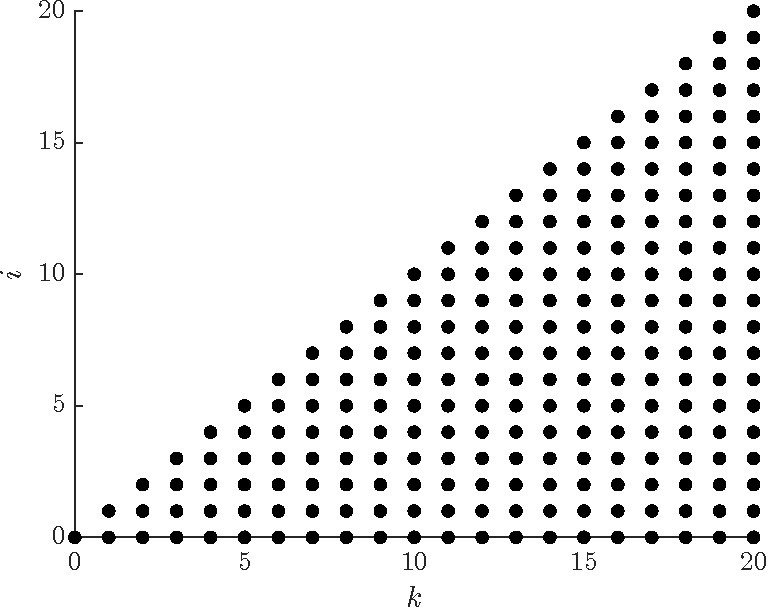
\includegraphics[width=0.5\textwidth]{supplements/ch2/ex2_17.pdf}
        \]
        Switching the order of summation and using the geometric series:
        \begin{align*}
            f(s) &= \prod_p \left\{\sum_{i=0}^\infty p^{iq}\sum_{k=i}^\infty \frac{1}{p^{ks}} \right\} = \prod_p \left\{\sum_{i=0}^\infty p^{i(q-s)}\sum_{k=0}^\infty \frac{1}{p^{ks}} \right\} \\
            \estepalign{\eqref{eq:power_geom}}  \prod_p \left\{\frac{1}{1-p^{q-s}}\frac{1}{1-p^{-s}}  \right\} \estep{\eqref{eq:power_zeta}}\zeta(s-q) \zeta(s) 
        \end{align*}
    \end{enumerate}
\end{solution}

\begin{exercise}
    \label{ex:2-18}
    For each of the following identities: first check that the identity is sometimes correct by calculating both sides of the alleged equation when $n=1,2,3,4,5,6,7,8$; next find the Dsgf's of the sequences on both sides of the claimed identity, observe that they are the same, and thereby prove the identity. Use the results of Exercise \ref{ex:2-16} above.
    \begin{enumerate}[label=(\alph*)]
        \item $\sum_{d\vert n} \phi(d) = n \quad (n\geq 1)$
        \item $\sum_{d\vert n} \mu(d) = 0$ if $n \geq 2$ and $= 1$ if $n=1$
        \item $\sum_{\delta\vert n} \mu(\delta)d(n/\delta) = 1 \quad (n\geq 1)$
    \end{enumerate}
\end{exercise}
\begin{solution}
    See Table \ref{tab:2:ex:2-18} for the calculated values of the left-hand sides of the claimed identities which are indeed the same as the alleged value.
    \begin{table}[hbpt]
        \centering
        \caption{Calculated values $n=1,2,\ldots,8$ for left-hand sides of identities.}
        \label{tab:2:ex:2-18}
        \begin{tabular}{@{}crrr@{}}
            \toprule 
            $n$ & $\sum_{d\vert n} \phi(d)$ & $\sum_{d\vert n} \mu(d)$ & $\sum_{\delta\vert n} \mu(\delta)d(n/\delta)$ \\ \midrule
            $1$ & $1 = 1$ & $1 = 1$ & $1\cdot 1 = 1$ \\
            $2$ & $1 + 1 = 2$ & $1 - 1 = 0$ & $1\cdot 2 - 1 \cdot 1 = 1$ \\
            $3$ & $1 + 2 = 3$ & $1 - 1 = 0$ & $1 \cdot 2 - 1 \cdot 1 = 1$ \\
            $4$ & $1 + 1 + 2 = 4$ & $ 1 - 1 + 0 = 0$ &  $1\cdot 3-1\cdot2+0\cdot 1=1$ \\
            $5$ & $1+ 4 = 5$& $1 - 1 =0$ &$1\cdot 2 - 1\cdot 1 = 1$ \\
            $6$ & $1+1+2+2 = 6$& $1-1-1+1=0$& $1 \cdot 4 - 1\cdot 2 -1\cdot 2 + 1\cdot 1 = 1$ \\
            $7$ & $1+6=7$&$1-1=0$ & $1\cdot 2 - 1 \cdot 1 = 1$\\
            $8$ & $1+1+2+4=8$ &$1-1+0+0=0$ & $1\cdot 4 - 1 \cdot 3 + 0 \cdot 2 + 0\cdot 1 = 1$\\
            \bottomrule
        \end{tabular}
    \end{table}

    The Dsgf's can be found using the identity:
    \[
        f(s) g(s) \stackrel{Dir}{\longleftrightarrow} \left\{\sum_{d\vert n}a_db_{\frac{n}{d}}\right\}_{n=1}^\infty
    \]
    for $f(s) \stackrel{Dir}{\longleftrightarrow} \{a_n\}_1^\infty$ and $g(s) \stackrel{Dir}{\longleftrightarrow} \{b_n\}_1^\infty$.
    \begin{enumerate}[label=(\alph*)]
        \item Dirichlet convolution of $\{1\}_1^\infty$ and $\{\phi(n)\}_1^\infty$:
        \[
            \zeta(s) \frac{\zeta(s-1)}{\zeta(s)} = \zeta(s-1)
        \]
        which is equal to the Dsgf of $\{n\}_1^\infty$ as found in Exercise \ref{ex:2-17}.
        \item Dirichlet convolution of $\{1\}_1^\infty$ and $\{\mu(n)\}_1^\infty$:
        \[
            \zeta(s) \frac{1}{\zeta(s)} = 1 = 1 + \frac{0}{2^s} + \frac{0}{3^s} + \ldots
        \]
        which is the Dsgf of the righ- hand side.
        \item Dirichlet convolution of $\{\mu(n)\}_1^\infty$ with $\{d(n)\}_1^\infty$ (where $d(n)$ is the divisor counting function with Dsgf $\zeta^2(s)$):
        \[
            \frac{1}{\zeta(s)} \zeta^2(s) = \zeta(s)
        \]
        which is the Dsgf of the right-hand side.
    \end{enumerate}
\end{solution}

\begin{exercise}
    Let $\{f(k)\}$ be the sequence of number of block fountains whose first row have $k$ coins with opsgf 
    \[
        F(x) = \frac{1-2x}{1-3x+x^2}
    \]
    Show that $f(k) = F_{2k-1}$ for $ k\geq 1$, where the $\{F_k\}$ are the Fibonacci numbers.
\end{exercise}
\begin{solution}
    Let the generating function of the Fibonacci numbers be $h(x)$:
    \[
        h(x) = \bsum[k] F_kx^k = \frac{x}{1-x-x^2}
    \]
    We search for a generating function for the odd numbers:
    \[
        \frac{h(x) - h(-x)}{2} = \bsum[k] F_{2k+1}x^{2k+1} \quad \Longleftrightarrow \quad
        \frac{h(x) - h(-x)}{2x} =\bsum[k] F_{2k+1}(x^2)^k
    \]
    Let $g(y)$ be the generating function for $F_{2k+1}$, then we have that:
    \[
        g(x^2) = \frac{1}{2(1-x-x^2)} + \frac{1}{2(1+x-x^2)} = \frac{1-x^2}{1-3x^2+x^4}
    \]
    from which $g(y)$ is evident. Because the generating function of $F_{2k-1}$ is equal to $yg(y)$:
    \[
        yg(y) = \bsum[k] F_{2k-1}y^k = \frac{y-y^2}{1-3y+y^2}
    \]
    For the opsgf of the block fountain sequence we have (subtract one to account for the differing value at $k=0$):
    \[
        F(x) - 1 = \frac{1-2x}{1-3x+x^2} - 1 = \frac{x-x^2}{1-3x+x^2}
    \]
    From the fact that the generating functions are equal, we can conclude that $f(k) = F_{2k-1}$ for $k\geq 1$.
\end{solution}

\begin{exercise}
    \label{ex:2-20}
    Prove the binomial theorem
    \[
        (x+y)^n = \sum_k\binom{n}{k}x^ky^{n-k}  
    \]
    by comparing the coefficient of $t^n/n!$ on both sides of the equation $e^{t(x+y)} = e^{tx}e^{ty}$. Prove the multinomial theorem
    \[
        (x_1+\cdots+x_k)^n = \sum_{r_1+\cdots+r_k=n} \frac{n!}{r_1!\cdots r_k!}x_1^{r_1}\cdots x_k^{r_k}
    \]
    by a similar device.
\end{exercise}
\begin{solution}
    Comparing the coefficient of $t^n/n!$ on both sides of the equation $e^{t(x+y)} = e^{tx}e^{ty}$:
    {\allowdisplaybreaks
    \begin{align*}
        \coeff{\frac{t^n}{n!}} e^{t(x+y)} &= \coeff{\frac{t^n}{n!}} e^{tx}e^{ty} \\
        \coeff{\frac{t^n}{n!}} \bsum[m] \frac{t^m(x+y)^m}{m!} &= \coeff{\frac{t^n}{n!}} \left(\bsum[m] \frac{t^mx^m}{m!}\right)\left( \bsum[k] \frac{t^ky^k}{k!}\right) \\
        (x+y)^n &= \coeff{\frac{t^n}{n!}} \bsum[m] \sum_{k=0}^m \frac{x^ky^{m-k}}{k!(m-k)!} t^m \\
        (x+y)^n &= \coeff{\frac{t^n}{n!}} \bsum[m] \sum_{k=0}^m \frac{m!}{k!(m-k)!} x^ky^{m-k}\frac{t^m }{m!} \\
        (x+y)^n &= \sum_{k=0}^n \binom{n}{k}x^ky^{n-k}
    \end{align*}
    }
    from which the binomial theorem follows.

    Similarly, for the multinomial theorem:
    \begin{align*}
        \coeff{\frac{t^n}{n!}} e^{t(x_1+\cdots + x_k)} &= \coeff{\frac{t^n}{n!}} \prod_{i=1}^k e^{tx_i} \\
        (x_1+\cdots+x_k)^n &= \coeff{\frac{t^n}{n!}} \bsum[m] \sum_{r_1+\cdots+r_k = m} \frac{x_1^{r_1}x_2^{r_2}\cdots x_k^{r_k}}{r_1!r_2!\cdots r_k!} t^m \\
        (x_1+\cdots+x_k)^n &= \coeff{\frac{t^n}{n!}} \bsum[m] \sum_{r_1+\cdots+r_k = m} \frac{m!}{r_1!r_2!\cdots r_k!} x_1^{r_1}x_2^{r_2}\cdots x_k^{r_k} \frac{t^m}{m!} \\
        (x_1+\cdots+x_k)^n &= \sum_{r_1+\cdots+r_k = n} \frac{n!}{r_1!r_2!\cdots r_k!} x_1^{r_1}x_2^{r_2}\cdots x_k^{r_k}
    \end{align*}
\end{solution}

\begin{exercise}
    \label{ex:2-21}
    \begin{enumerate}[label=(\alph*)]
        \item Let $T$ be a fixed set of nonnegative integers. Let $f(n,k,T)$ be the number of ordered representations of $n$ as a sum of $k$ integers chosen from $T$. Find $\sum_n f(n,k,T)x^n$.
        \item Let $g(n,k,T)$ be the number of ordered represenations of $n$ as a sum of $k$ \emph{distinct} integers chosen from $T$. Find $\sum_n g(n,k,T)x^n$.
        \item Finally, let $S$, $T$ be two fixed sets of nonnegative integers. Let $f(n,k,S,T)$ be the number of ordered representations of $n$ as a sum of $k$ integers chosen from $T$, each being chosen with a multiplicity that belongs to $S$. Find $\sum_n f(n,k,S,T)x^n$.
    \end{enumerate}
\end{exercise}
\begin{solution}
    \begin{enumerate}[label=(\alph*)]
        \item The opsgf is given by the $k$th power of $\sum_{t\in T} x^t$. Indeed:
        \[
            \left(\sum_{t\in T} x^t\right)^k = \bsum x^n  \sum_{\substack{t_i \in T \\ \sum_{i=1}^k t_i = n}} 1 = \bsum x^n f(n,k,T)
        \]
        The interpretation of this opsgf is that for each index from $1$ to $k$ we choose a number from $T$.
        \item Instead of choosing a number from $T$ for each index, we now choose for each number from $T$ whether we take it or not. This leads to the `building block':
        \[
            (1 + x^t)
        \]
        which corresponds to not taking and taking $t$ respectively. Taking the product:
        \begin{align*}
            \prod_{t\in T} (1+x^t)
        \end{align*}
        gives the opsgf of the number of unordered ways a number can be written as a sum of distinct integers from $T$. 
        
        To find the number of ways with exactly $k$ distinct integers, multiply $x^t$ with $y$ and then take the coefficient of $y^k$. By doing this, each time a number $t$ is taken, the coefficient of $y$ is also incremented. Therefore, the coefficient corresponding to $y^k$ will have exactly chosen $k$ values:
        \begin{align*}
            \coeff{y^k} \prod_{t\in T} (1+yx^t)
        \end{align*}
        However, this is the number of unordered ways. To count the number of ordered ways, it suffices to multiply with $k!$ since each permutation is another way (assuming the $t \in T$ are distinct):
        \[
            \bsum g(n,k,T)x^n = \coeff{y^k} k! \prod_{t\in T} (1+yx^t)
        \]
        \item Similarly, we choose for each number from $T$ which multiplicity we want to take from $S$ which leads to the building block:
        \[
            \sum_{s \in S} x^{st}
        \]
        After making all choices:
        \[
            \prod_{t\in T} \sum_{s \in S} x^{st}
        \]
        Again, to take $k$ integers, we multiply with $y^s$ and then take the coefficient of $y^k$. To take into account the fact that the numbers are not labeled we also divide by $\frac{1}{s!}$ since all these permutations are the same:
        \[
            \coeff{y^k} \prod_{t\in T} \sum_{s \in S} \frac{y^sx^{st}}{s!}
        \]
        Now, taking all permutations of the chosen $k$ integers (note that the fact that all $s$ values of a number are indistinguishable is already accounted for by $\frac{1}{s!}$):
        \[
            \bsum f(n,k,S,T)x^n = \coeff{y^k} k!\prod_{t\in T} \sum_{s \in S} \frac{y^sx^{st}}{s!}
        \]
    \end{enumerate}
\end{solution}

\begin{exercise}
    Let $f(n)$ be the excess of the number of ordered represenations of $n$ as the sum of an even number of positive integers over those as a sum of an odd number of them. Find $f(n)$ by finding $\sum_n f(n)x^n$ and reading off its coefficients.
\end{exercise}
\begin{solution}
    The number of ways of writing $n$ as a sum of $k$ positive integers ($> 0$) is the coefficient of $x^n$ in the opsgf of:
    \[
        (x + x^2 + \ldots )^k = \left(\frac{x}{(1-x)}\right)^k
    \]
    The excess number of ordered representations of $n$ as the sum of an even number of positive numbers over those of a sum of an odd number of them is therefore:
    \[
        \bsum f(n) x^n = \sum_{k=1}^\infty (-1)^k \frac{x^k}{(1-x)^k} \estep{\eqref{eq:power_geom}} \frac{1}{1 - \frac{-x}{1-x}} - 1 = \frac{1-x}{1} - 1 = -x
    \]
    from which we can see that $f(1) = -1$ and $f(n) = 0$ for all $n > 1$.
\end{solution}

\begin{exercise}
    Let $\{B_n\}$ be the sequence of Bernoulli numbers defined by \eqref{eq:power_bernoulli} and let $m$ be a positive integer. By considering the generating function
    \[
        \frac{x(e^{mx}-1)}{e^x-1}
    \]
    in two ways, find an evaluation of the sum of the $r$th powers of the first $N$ positive integers as a polynomial of degree $r+1$ in $N$, whose coefficients are given quite explicitly in terms of the Bernoulli numbers.
\end{exercise}
\begin{solution}
    First of all, using the definition of the Bernoulli numbers as well as the power series for the exponential:
    \[
        \frac{x}{e^x - 1}(e^{mx} - 1) \estep{\eqref{eq:power_bernoulli}, \eqref{eq:power_exp}} \bsum \frac{B_n x^n}{n!} \sum_{k=1}^\infty \frac{m^kx^{k}}{k!}
    \] 
    Setting $j=n+k$:
    \begin{align*}
        \frac{x}{e^x-1}(e^{mx} - 1) &= \sum_{j=1}^\infty x^j \left(\sum_{k=1}^j \frac{m^kB_{j-k}}{(j-k)!k!}\right) = \sum_{j=1}^\infty \frac{x^j}{j!} \left(\sum_{k=1}^\infty \binom{j}{k}m^kB_{j-k}\right)
    \end{align*}
    Note that in the last step we also used the fact that $\binom{j}{k}=0$ for $k>j$ to extend the range of summation.
    Secondly, a geometric series is also recognized:
    \[
        x\frac{e^{mx} - 1}{e^x - 1} = x \sum_{k=0}^{m-1} e^{kx} \estep{\eqref{eq:power_exp}} x \sum_{k=0}^{m-1} \bsum[j] \frac{k^jx^j}{j!}
    \]
    Switching the order of summation:
    \[
        x\frac{e^{mx} - 1}{e^x - 1} = \bsum[j] \frac{x^{j+1}}{j!} \sum_{k=0}^{m-1} k^j = \bsum[j] \frac{x^{j+1}}{j!} S_j(m-1) = \sum_{j=1}^\infty \frac{x^j}{(j-1)!} S_{j-1}(m-1)
    \]
    where $S_j(m)$ is the sum of the $j$th powers of $1, 2, \ldots, m$. Comparing the coefficients of $x^n$ gives:
    \[
        \frac{S_{n-1}(m-1)}{(n-1)!} = \frac{1}{n!} \sum_{k=1}^\infty \binom{n}{k}m^k B_{n-k}
    \]
    which is equivalent to:
    \[
        (n+1)S_n(m) = \sum_{k=1}^\infty \binom{n+1}{k} (m+1)^k B_{n-k+1} = \sum_{k=1}^{n+1} \binom{n+1}{k} (m+1)^k B_{n-k+1}
    \]
    which is a polynomial of degree $n+1$ in $m$.
\end{solution}

\begin{exercise}
    \label{ex:2-24}
    \begin{enumerate}[label=(\alph*)]
        \item Make a table of values of the classical M{\"o}bius function $\mu(n)$ for $n=1,2,\ldots,30$.
        \item Make a table of the values of the function $f(n)$ of 
        \[
            f(n) = \sum_{d\vert n}\mu\left(\frac{n}{d}\right)2^d \qquad (n=1,2,\ldots)
        \]
        for $n=1,2,\ldots,12$.
        \item Make a list of the primitive strings of length $6$, and verify your value of $f(6)$.
    \end{enumerate}
\end{exercise}
\begin{solution}
    \begin{enumerate}[label=(\alph*)]
        \item See Table \ref{tab:ex:2-24}
        \item See Table \ref{tab:ex:2-24}
        \item The list of primitive strings of length $6$ is:
        \begin{align*}
            &000001,\ 000010,\ 000011,\ 000100,\ 000101,\ 000110\ \\ &000111,\ 001000,\  001010,\ 001011,\ 001100,\ 001101\ \\ &001110,\ 001111,\ 010000,\ 010001,\ 010011,\ 010100\ \\&010110,\ 010111,\ 011000,\ 011001,\ 011010,\ 011100\ \\& 011101,\ 011110,\ 011111,\ 100000,\ 100001,\ 100010\ \\&100011,\ 100101,\ 100110,\ 100111,\ 101000,\ 101001\ \\&101011,\ 101100,\ 101110,\ 101111,\ 110000,\ 110001\ \\&110010,\ 110011,\ 110100,\ 110101,\ 110111,\ 111000\ \\&111001,\ 111010,\ 111011,\ 111100,\ 111101,\ 111110
        \end{align*}
        which is indeed of length $54$.
    \end{enumerate}
    \begin{table}[hbpt]
        \centering
        \caption{Solution Exercise \ref{ex:2-24}.}
        \label{tab:ex:2-24}
        \begin{tabular}{@{}c@{\quad}c@{\qquad\qquad}c@{}}
            \begin{tabular}{@{}rr@{}}
                \toprule 
                $n$ & $\mu(n)$ \\ \midrule
                $1$ & $1$ \\
                $2$ & $-1$\\ 
                $3$ & $-1$\\  
                $4$ & $0$\\  
                $5$ & $-1$\\  
                $6$ & $1$\\  
                $7$ & $-1$\\  
                $8$ & $0$\\ 
                $9$ & $0$\\
                $10$ & $1$\\ 
                $11$ & $-1$\\ 
                $12$ & $0$\\  
                $13$ & $-1$ \\
                $14$ & $1$ \\
                $15$ & $1$ \\ \bottomrule
            \end{tabular} &
            \begin{tabular}{@{}rr@{}}
                \toprule
                $n$ & $\mu(n)$ \\ \midrule
                $16$ & $0$ \\
                $17$ & $-1$ \\
                $18$ & $0$ \\
                $19$ & $-1$\\
                $20$ & $0$ \\
                $21$ & $1$ \\
                $22$ & $1$\\
                $23$ & $-1$  \\
                $24$ & $0$ \\
                $25$ & $0$\\
                $26$ & $1$ \\
                $27$ & $0$ \\
                $28$ & $0$\\
                $29$ & $-1$ \\
                $30$ & $-1$ \\ \bottomrule
            \end{tabular} & 
            \begin{tabular}{@{}rr@{}}
                \toprule
                $n$ & $f(n)$ \\ \midrule
                $1$ & $2$\\
                $2$ & $2$\\
                $3$ & $6$\\
                $4$ & $12$\\
                $5$ & $ 30$\\
                $6$ & $54$\\
                $7$ & $126$\\
                $8$ & $240$\\
                $9$ & $504$ \\
                $10$ & $990$\\
                $11$ & $2046$\\
                $12$ & $4020$
                \\ \bottomrule
            \end{tabular}
        \end{tabular}
    \end{table}
\end{solution}

\begin{exercise} \label{ex:2-25}
    This exercise is intended to show how generating functions occur in coding theory. An important question is the following: for fixed integers $n$ and $d$, what is the length $A(n,d)$ of the longest list of $n$-bit strings of $0$'s and $1$'s (\emph{codewords}) such that two distinct codewords always differ in at least $d$ bit positions?
    \begin{enumerate}[label=(\alph*)]
        \item Assign to each of the $2^n$ codewords $(\epsilon_1,\ldots,\epsilon_n)$ a \emph{color}, as follows: the color of $\epsilon$ is $\sum_j j \epsilon_j$ modulo $2n$. Show that if two codewords differ in just $1$ or $2$ coordinates, then they are assigned distinct colors in this scheme.
        \item From part (a), show that $A(n,3) \geq 2^n /(2n)$.
        \item Let $a_j$ be the number of codewords for which $\sum_r r\epsilon_r = j$, for each $j$. Find the opsgf $f(z) = \sum_j a_jz^j$ explicitly as a product.
        \item If $\beta_r$ is the number of codewords of color $r$, then express $\beta_r$ in terms of the $a_j$'s above. Then use the roots of unity method to find that 
        \[
            \beta_r = \frac{1}{2n}\sum_{j=1}^{n''} 2^{2^a(j,n'')}e^{-\frac{2\pi irj}{n''}}
        \]
        for each $r = 0,1,\ldots,2n-1$. Here $a$ and $n''$ are defined by $n=2^an''$ where $n''$ is odd, and $(b,c)$ denotes the gcd of $b$ and $c$.
        \item Deduce that $\beta_0$ is the largest of the $\beta_r$'s, and therefore find the stronger bound
        \[
            A(n,3) \geq \frac{1}{2n} \sum_{j=1}^{n''}2^{2^a(j,n'')} \geq \frac{2^n}{2n}.
        \]
        \item Use Parseval's identity and the result of part (d) to find the variance of the occupancy numbers $\beta_0,\ldots,\beta_{2n-1}$. Make an estimate that shows that the variance is in some sense very small, so that this coloring scheme is shown to distribute codewords into color classes very uniformly.
    \end{enumerate}
\end{exercise}
\begin{solution}
    \begin{enumerate}[label=(\alph*)]
        \item If the codewords differ in the $j$th coordinate, the difference between the colors will be $j$ which means that the assigned color is different ($j \leq n$). 
        
        If the codewords differ in the $j$th and the $k$th coordinate, the difference between the color values is either $j+k$ or $j-k$, both of which are smaller than $2n$ and therefore the codewords can't be in the same class.
        \item From the pigeonhole principle, there exists a color with at least $2^n/(2n)$ elements. These elements differ in at least $3$ elements (since otherwise they would have distinct colors). Therefore:
        \[
            A(n,3) \geq \frac{2^n}{2n}  
        \]
        \item Each bit either contributes $0$ or $r$ to the sum (where $r$ is the index ranging from $1$ to $n$). Therefore the opsgf is:
        \[
            f(z) = \bsum[j] a_j z^j = \prod_{k=1}^n (1 + z^k)
        \]
        \item $\beta_r$ is the number of codewords of color $r$. This corresponds to summing all coefficients for the powers with the same value modulo $2n$:
        \[
            \beta_r = \bsum[k] a_{r+2nk} = \bsum[k] a_{r+2nk}z^{r+2nk} \Bigr\vert_{z=1} = g(z) \Bigr\vert_{z=1}
        \]
        for some $g(z)$. We then choose $g(z)$ as follows and check that it is indeed the correct choice.
        \[
            g(z) = \frac{1}{2n} \sum_{l=0}^{2n-1} \frac{f(\omega_{2n}^lz)}{\omega_{2n}^{lr}}
        \]
        with $\omega_{2n}^l$ a $2n$th root of unity $e^{\frac{2\pi il}{2n}} = e^{\frac{\pi il}{n}}$. Working this out, we find:
        \[
            g(z) = \frac{1}{2n} \sum_{l=0}^{2n-1} \bsum[j] a_j \omega_{2n}^{l(j-r)}z^{j} = \frac{1}{2n} \bsum[j] a_jz^{j} \sum_{l=0}^{2n-1} \omega_{2n}^{l(j-r)}
        \]
        The last summation is $2n$ if and only if $j-r$ is a multiple of $2n$ and $0$ otherwise, therefore set $j = 2kn +r$ with $k=0,1,\ldots$:
        \[
            g(z) = \bsum[k] a_{2kn+r}z^{2kn+r}
        \]
        which is indeed what we were after. Evaluating $g(z)$ at $z=1$ will give the desired $\beta_r$. We now fill in the found $f(z)$ from part (c):
        \[
            \beta_r = g(1) = \frac{1}{2n} \sum_{l=0}^{2n-1} \frac{f(\omega_{2n}^l)}{\omega_{2n}^{lr}} = \frac{1}{2n} \sum_{l=0}^{2n-1} \frac{1}{\omega_{2n}^{lr}} \prod_{k=1}^n (1 + \omega_{2n}^{lk})
        \]
        Taking out the first term from the summand yields
        \[
            \beta_r = \frac{2^n}{2n} + \frac{1}{2n}\sum_{l=1}^{2n-1} \frac{1}{\omega_{2n}^{lr}} \prod_{k=1}^n (1+\omega_{2n}^{lk})
        \]
        Now note that we can omit all terms from the sum where the product evaluates to zero. The product evaluates to zero if $\omega_{2n}^{lk} = -1$, i.e., $e^{\frac{i\pi l k}{n}} = -1$ which is when $\frac{lk}{n}$ is an odd number. Now suppose $\gcd(l,n) = d$ and take $k = \frac{n}{d}$, then the term is definitely zero when $\frac{lk}{n} = \frac{l}{d}$ is an odd number.
        
        Now define $n''$ and $a$ such that $n=2^an''$ where $n''$ is odd (separating the prime factor two with its exponent from $n$). Suppose the exponent of 2 in the prime factorization of $l$ is $b \leq a$. Then $\frac{l}{\gcd(l,n)}$ will be odd (because the factors of two will cancel). All these terms can therefore be omitted. We now only iterate over multiples of $2^{a+1}$ for $l$. The maximum multiple corresponds to a factor $n''-1$. Indeed for $n''$ we would have $n'' 2^{a+1} = 2n''2^a = 2n > 2n-1$. Using these observations we now write:
        \begin{align*}
            \beta_r &= \frac{2^n}{2n} + \frac{1}{2n}\sum_{j=1}^{n''-1} \exp\left(\frac{-2^{a+1}ijr\pi}{n}\right) \left\{\prod_{k=1}^n \left(1 + \exp\left(\frac{2^{a+1}ijk\pi}{n}\right)\right)\right\}
        \end{align*}
        Using the fact that $n=2^an''$:
        \begin{align*}
            \beta_r &= \frac{2^n}{2n} + \frac{1}{2n}\sum_{j=1}^{n''-1} \exp\left(\frac{-2ijr\pi}{n''}\right)  \left\{\prod_{k=1}^n \left(1 + \exp\left(\frac{2ijk\pi}{n''}\right)\right)\right\}
        \end{align*}
        Bring out the first term back into the sum as index $j = n''$ (the complex exponentials evaluate to $1$):
        \[
            \beta_r = \frac{1}{2n}\sum_{j=1}^{n''}\exp\left(\frac{-2ijr\pi}{n''}\right)  \left\{\prod_{k=1}^n \left(1 + \exp\left(\frac{2ijk\pi}{n''}\right)\right)\right\}
        \]
        The inner exponential is equal up to modulo $n''$ due to the periodicity of the exponential:
        \[
            \exp\left(\frac{2ij(k' + k''n'')\pi}{n''}\right) = \exp\left(\frac{2ijk'\pi}{n''}\right)
        \] Therefore only $k$ values $1,2,\ldots,n''$ need to be considered with each term occuring $2^a$ times:
        \[
            \beta_r = \frac{1}{2n}\sum_{j=1}^{n''} \exp\left(\frac{-2ijr\pi}{n''}\right) \left\{\prod_{k=1}^{n''} \left(1 + \exp\left(\frac{2ijk\pi}{n''}\right)\right)^{2^a}\right\}
        \]
        Similarly, for each $j$ value, the exponential is equal up to modulo $\frac{n''}{\gcd(j,n'')}$ due to the periodicity: 
        \begin{align*}
            \exp\left(\frac{2ij\left(k' + \frac{k''n''}{\gcd(j,n'')}
                \right)\pi}{n''}\right) = \exp\left(\frac{2ijk'\pi}{n''} + \cancel{\frac{2ij\pi}{\gcd(j,n'')}}\right)
        \end{align*}
        We now have:
        \[
            \beta_r = \frac{1}{2n}\sum_{j=1}^{n''} \exp\left(\frac{-2ijr\pi}{n''}\right)  \left\{\prod_{k=1}^{\frac{n''}{\gcd(j,n'')}} \left(1 + \exp\left(\frac{2ijk\pi}{n''}\right)\right)^{2^a\gcd(j,n'')}\right\}
        \]
        Note that the product contains a permutation of roots of unity of order $\frac{n''}{\gcd(j,n'')}$  since:
        \[
            \exp\left(\frac{2ij\pi}{n''}\right) = \exp\left(\frac{\frac{2ij\pi}{\gcd(j,n'')}}{\frac{n''}{\gcd(j,n'')}}\right)
        \]
        where numerator and denominator are coprime which means that it is a primitive root of unity and therefore therefore generates all others. Define $m= \frac{n''}{\gcd(j,n'')}$ such that we are searching for:
        \[
            \prod_{k=1}^m (1 + \omega_m^k)
        \]
        Now consider the polynomial:
        \[
            \prod_{k=1}^{m} (x-(1+\omega_m^k)) = \prod_{k=1}^{m} ((x-1)-\omega_m^k)
        \]
        whose constant term is given by:
        \[
            \coeff{x^0}\prod_{k=1}^{m} (x-(1+\omega_m^k)) = (-1)^m \prod_{k=1}^{m}(1+\omega_m^k)
        \]
        which is exactly what we are searching for.

        Because the roots of unity are solutions of $z^m = 1$, the factorisation of $z^m - 1 = \prod_{k=1}^m (z - \omega_m^k)$. Substituting $z = (x-1)$, we find:
        \[
            \prod_{k=1}^{m} ((x-1)-\omega_m^k) = (x-1)^m - 1
        \]
        with constant term:
        \[
            \coeff{x^0} (x-1)^m - 1 = (-1)^m - 1
        \]
        Now, because $n''$ is odd by construction, we also have that $m$ is odd:
        \[
            \prod_{k=1}^m (1 + \omega_m^k) = (-1)^m((-1)^m - 1) = -(-1 - 1) = 2
        \]
        Filling this back into the equation for $\beta_r$ gives the desired expression:
        \[
            \beta_r = \frac{1}{2n} \sum_{j=1}^{n''} \exp\left(\frac{-2ijr\pi}{n''}\right) 2^{2^a \gcd(j,n'')}
        \]
        \item To show that $\beta_r \leq \beta_0$ for all $r$, the triangle inequality is used:
        \[
            |\beta_r| = \left|\frac{1}{2n} \sum_{j=1}^{n''}e^{\frac{-2ijr\pi}{n''}} 2^{2^a \gcd(j,n'')}\right| 
            \leq \frac{1}{2n} \sum_{j=1}^{n''} 2^{2^a \gcd(j,n'')} = \beta_0
        \]
        Because there are $\beta_0$ numbers in that class, we have that $A(n,3) \geq \beta_0$ by the same argument as part (b). Now to show that the bound is stronger than the previous bound we take out the last term of the sum:
        \[
            \beta_0 =  \frac{1}{2n} \sum_{j=1}^{n''} 2^{2^a \gcd(j,n'')} = \frac{2^{2^a\gcd(n'',n'')}}{2n} + \frac{1}{2n}   \sum_{j=1}^{n''-1}2^{2^a \gcd(j,n'')}
        \]
        Since $n=n''2^a$:
        \[
            \beta_0 = \frac{2^n}{2n} +\frac{1}{2n}   \sum_{j=1}^{n''-1}2^{2^a \gcd(j,n'')} \geq \frac{2^n}{2n} 
        \] and we have:
        \[
            A(n,3) \geq \beta_0 \geq \frac{2^n}{2n}
        \]
        \item First of all, note that $\beta_r$ is $n''$-periodic. Indeed:
        \[
            \beta_{r + kn''} = \frac{1}{2n}\sum_{j=1}^{n''}e^{\frac{-2ij(r+kn'')\pi}{n''}} 2^{2^a \gcd(j,n'')}  = \beta_r
        \]
        The summation can therefore be written with lower bound $0$ and upper bound $n''-1$ since the term corresponding to $n''$ is equal to the $0$th term.
        \[
            \beta_r = \frac{1}{2n}\sum_{j=1}^{n''}e^{\frac{-2ijr\pi}{n''}} 2^{2^a \gcd(j,n'')} = \frac{1}{2n}\sum_{j=0}^{n''-1}e^{\frac{-2ijr\pi}{n''}} 2^{2^a \gcd(j,n'')}
        \]

        Now consider the $n''$ numbers $2^{2^a\gcd(0,n'')}, \ldots, 2^{2^a\gcd(n''-1,n'')}$ with discrete Fourier transform:
        \[
            X_k = \sum_{l=0}^{n''-1} 2^{2^a\gcd(l,n'')}e^{-\frac{2i\pi kl}{n''}} = 2n\beta_k
        \]
        From Parseval's identity, we therefore have:
        \[
            \sum_{l=0}^{n''-1} \left|2^{2^a\gcd(l,n'')}\right|^2 = \frac{1}{n''}\sum_{k=0}^{n''-1} |2n\beta_k|^2
        \]
        Switching sides yields:
        \[
            \frac{4n^2}{n''}\sum_{k=0}^{n''-1} \beta_k^2 = \sum_{l=0}^{n''-1} 2^{2^{a+1}\gcd(l,n'')}
        \]
        Now, the variance of the occupancy numbers is:
        \begin{align*}
            \sigma^2 &= \frac{1}{2n} \sum_{k=0}^{2n-1} (\beta_k - \mu)^2
        \end{align*}
        Where $\mu$ is the mean which is equal to $\frac{2^n}{2n}$ since the occupancy numbers sum up to $2^n$. Simplifying gives:
        \[
            \sigma^2 = \frac{1}{2n}\left(\sum_{k=0}^{2n-1} \beta_k^2\right) - \mu^2  = \frac{1}{2n}\left(2^{a+1}\sum_{k=0}^{n''-1} \beta_k^2\right) - \mu^2
        \]
        where in the last equality, we used that $\beta_r$ is $n''$-periodic with each term occuring $2^{a+1}$ times.
        Applying the result from Parseval's identity:
        \[
            \sigma^2 = \frac{1}{2n}\left(\frac{n''2^{a+1}}{4n^2} \sum_{l=0}^{n''-1} 2^{2^{a+1}\gcd(l,n'')}\right) - \mu^2 = \frac{1}{4n^2}\sum_{l=0}^{n''-1} 2^{2^{a+1}\gcd(l,n'')} - \mu^2
        \]
        The term for $l=0$ equals $2^{2n}$ meaning that it can be cancelled with $\mu^2$:
        \[
            \sigma^2 = \frac{1}{4n^2}\sum_{l=1}^{n''-1} 2^{2^{a+1}\gcd(l,n'')}
        \]
        This variance is bounded by:
        \[
            \sigma^2 \leq \frac{1}{4n^2} \sum_{l=1}^{n'' - 1} 2^{2^{a+1} \frac{n''}{3}} \leq \frac{n''}{4n^2} 2^{\frac{2n}{3}} \leq \frac{2^{\frac{2n}{3}}}{4n}
        \]
        The first inequality follows from the fact that the gcd is bounded by $\frac{n''}{3}$ for $l$ between $1$ and $n''-1$ (also taking into account the fact that $n''$ is odd).

        Now, this variance is small in the relative sense with respect to $\mu$.
        \[
            \frac{\sigma}{\mu} \leq \frac{\frac{2^{\frac{n}{3}}}{2\sqrt{n}}}{\frac{2^{n}}{2n}} = \sqrt{n}2^{\frac{-2n}{3}}
        \]
    \end{enumerate}
\end{solution}

\begin{exercise}
    Show that:
    \[
        \binom{-n}{k} = (-1)^k\binom{n+k-1}{k}
    \]
\end{exercise}
\begin{solution}
    The right-hand side is given by
    \[
        (-1)^k \binom{n+k-1}{k} = (-1)^k \frac{\prod_{i=0}^{k-1} (n+k-1-i)}{k!} = (-1)^k \frac{\prod_{i'=0}^{k-1} (n+i')}{k!}
    \]
    Pulling the $(-1)$ inside yields the identity:
    \[
        (-1)^k\binom{n+k-1}{k} = \frac{\prod_{i'=0}^{k-1} (-n-i')}{k!} = \binom{-n}{k}
    \]
\end{solution}

\begin{exercise}
    \label{ex:2-27}
    Let $D(n)$ be the number of derangements of $n$ letters.
    \begin{enumerate}[label=(\alph*)]
        \item Find, in simple explicit form, the egf of $\{D(n)\}_0^\infty$.
        \item Prove, by any method, that
        \[
            D(n+1)=(n+1)D(n)+ (-1)^{n+1} \qquad (n\geq0;\ D(0)=1)
        \]
        \item Prove, by any method, that
        \[
            D(n+1) = n(D(n) + D(n-1)) \qquad (n\geq 1;\ D(0)=1;\ D(1)=0)
        \]
        \item Show that the number of permutations of $n$ letters that have exactly one fixed point differs from the number with no fixed points by $\pm 1$.
        \item Let $D_k(n)$ be the number of permutations of $n$ letters that have exactly $k$ fixed points. Show that
        \[
            \sum_{k,n\geq0} D_k(n)\frac{x^ny^k}{n!} = \frac{e^{-x(1-y)}}{1-x}.  
        \]
    \end{enumerate}
\end{exercise}
\begin{solution}
    \begin{enumerate}[label=(\alph*)]
        \item \hypertarget{eq:ch2:27:a}{} The numbers $D(n)$ satisfy the recurrence:
        \[
            n! = \bsum[k] \binom{n}{k} D_{n-k} \qquad(n\geq0)
        \]
        Taking the egf of both sides gives:
        \[
            \frac{1}{1-x} = e^xD(x) \Longleftrightarrow D(x) = \frac{e^{-x}}{(1-x)}
        \]
        such that
        \[
            D(n) = \coeff{\frac{x^n}{n!}} \bsum[m] \frac{(-x)^m}{m!} \bsum[k] x^k = \coeff{\frac{x^n}{n!}}\sum_{l=0}^\infty\sum_{k=0}^l  \frac{(-1)^kx^{l}}{k!} = n! \sum_{k=0}^n \frac{(-1)^k}{k!}
        \]
        where we used \eqref{eq:power_geom}, \eqref{eq:power_exp} in the first equality.
        \item \hypertarget{eq:ch2:27:b}{} Using the found expression for $D(n)$:
        \[
            (n+1)D(n) = (n+1)n!\sum_{k=0}^n \frac{(-1)^k}{k!}
            = (n+1)!\sum_{k=0}^n \frac{(-1)^k}{k!}
        \]
        Adding and subtracting $(-1)^{n+1}/(n+1)!$ inside:
        \[
            (n+1)D(n) = (n+1)! \left(-\frac{(-1)^{n+1}}{(n+1)!} + \sum_{k=0}^{n+1} \frac{(-1)^k}{k!}\right) = (-1)^{n} + D(n+1)
        \]
        After rearranging:
        \[
            D(n+1) = D(n)(n+1) + (-1)^{n+1}
        \]

        \item Applying the previous recurrence twice gives:
        \begin{align*}
            D(n+1) &= D(n)(n+1) + (-1)^{n+1} \\
            &= nD(n) + D(n) + (-1)^{n+1} \\
            &= nD(n) + nD(n-1) + (-1)^{n} + (-1)^{n+1}
        \end{align*}
        The two $-1$ terms will cancel each other since one will be $1$ and the other $-1$ such that we find:
        \[
            D(n+1) = n(D(n) + D(n-1))
        \]
        \item Number of permutations of $n$ letters with exactly $1$ fixed point equals the number of derangements $D(n-1)$ times $n$ (for all possibilities of the fixed point).
        
        Taking the difference with $D(n)$ gives:
        \[
            D(n) - nD(n-1) = (-1)^n
        \]
        by part \hyperlink{eq:ch2:27:b}{(b)}, so the difference is $\pm 1$.
        \item Similarly, $D_k(n)$ is given by $D(n-k)\binom{n}{k}$ since there are $\binom{n}{k}$ to choose the fixed points. Multiplying by $\frac{x^ny^k}{n!}$ and summing:
        \begin{align*}
            \sum_{k,n\geq 0} D_k(n) \frac{x^ny^k}{n!} &= \bsum[k]\bsum[n] \binom{n}{k} D(n-k) \frac{x^ny^k}{n!} \\
            &= \bsum  \frac{x^n}{n!} \bsum[k] \binom{n}{k}D(n-k) y^k \\
            \estepalign{\hyperlink{eq:ch2:27:a}{2.27(a)}, \eqref{eq:power_exp}} \bsum \frac{x^n}{n!} \bsum[k] \binom{n}{k} \coeff{\frac{x^{n-k}}{(n-k)!}} \left\{\frac{e^{-x}}{(1-x)}\right\} \coeff{\frac{x^k}{k!}} e^{xy}
        \end{align*}
        A multiplication of two egfs is recognized:
        \[
            \sum_{k,n\geq0} D_k(n) \frac{x^ny^k}{n!} = \bsum \frac{x^n}{n!} \left(\coeff{\frac{x^n}{n!}} \left\{\frac{e^{-x(1-y)}}{1-x} \right\}\right) = \frac{e^{-x(1-y)}}{1-x}
        \]
    \end{enumerate}
\end{solution}

\begin{exercise}
    \label{ex:2-28}
    Prove the following variation of the M{\"o}bius inversion formula. Let $\{a_n(x)\}$ and $\{b_n(x)\}$ be two sequences of functions that are connected by the relation
    \[
        a_n(x)= \sum_{d \vert n} b_{\frac{n}{d}}(x^d) \qquad (n=1,2,3,\dots).  
    \]
    Then we have
    \[
        b_n(x) = \sum_{d\vert n} \mu\left(\frac{n}{d}\right) a_d(x^{n/d}) \qquad (n=1,2,3,\ldots).  
    \]
\end{exercise}
\begin{solution}
    Starting from the right hand side of the asked identity and substituting the definition of $a_n(x)$:
    \[
        \sum_{d\vert n}  \mu\left(\frac{n}{d}\right) a_d(x^{n/d}) =  \sum_{d\vert n}  \mu\left(\frac{n}{d}\right) \sum_{d' \vert d} b_{\frac{d}{d'}}(x^{nd'/d}) 
    \]
    \[
       \Longleftrightarrow \sum_{d\vert n}  \mu\left(\frac{n}{d}\right) a_d(x^{n/d}) =  \sum_{d\vert n} \sum_{d' \vert d} b_{\frac{d}{d'}}(x^{nd'/d}) \mu\left(\frac{n}{d}\right) 
    \]
    Assume that $n=\frac{n}{d}d = \frac{n}{d}\frac{d}{d'}d' = khd'$ where $k=\frac{n}{d}$ and $h=\frac{d}{d'}$. We then have
    \[
        \sum_{d\vert n}  \mu\left(\frac{n}{d}\right) a_d(x^{n/d}) =  \sum_{kd=n} \sum_{hd'=d} b_{h}(x^{n/h}) \mu\left(k\right) = \sum_{khd' = n}b_{h}(x^{n/h}) \mu\left(k\right)
    \]
    where the subscript means that we iterate over all triplets $(k,h,d')$ (or pairs) such that the relation is satisfied. This is equivalent to first choosing the divisor $h$ of $n$ and then choosing $k$ to be a divisor of $\frac{n}{h}$ (then $d'$ is fixed), i.e.\
    \[
        \sum_{d\vert n}  \mu\left(\frac{n}{d}\right) a_d(x^{n/d}) = \sum_{h\vert n}b_h(x^{n/h}) \sum_{k \vert \frac{n}{h}} \mu(k)
    \]
    The summation over $\mu(k)$ is a Dirichlet convolution with the Riemann zeta function and results in $1$ if and only if $\frac{n}{h} = 1$ and $0$ otherwise (see also Exercise \ref{ex:2-18}(b)). This means that $h = n$ is the only remaining term:
    \[
        \sum_{d\vert n}  \mu\left(\frac{n}{d}\right) a_d(x^{n/d}) = b_n(x)
    \]
\end{solution}

\begin{exercise}
    \begin{enumerate}[label=(\alph*)]
        \item Make a table of the values $\phi(n)$ for $1\leq n\leq 25$.
        \item As far as your table goes, verify that $\phi(n)$ is a multiplicative function, by actual computation. Then check by actual computation from your table, that the result stated in Exercise \ref{ex:2-14} above is true when $n=20$ and $n=24$.
        \item Let $n=p^\alpha$ where $p$ is a prime number. What is $\phi(n)$?
        \item Use the results above to find a general formula for $\phi(n)$ in terms of the prime factorization $n=p_1^{\alpha_1}p_2^{\alpha_2}\cdots p_k^{\alpha_k}$ of $n$. Use your results to calculate $\phi(2592)$.
        \item Find the Dirichlet series generating function of $\phi(n)$, using Theorem \ref{thm:euler_prod}, and express it in terms of the Riemann zeta function.
        \item Apply the M{\"o}bius inversion formula to the result of Exercise \ref{ex:2-18}(a), and thereby ``solve'' \ref{ex:2-18}(a) for $\phi(n)$, to get an explicit formula for $\phi(n)$ that involves a sum of various values of the M{\"o}bius function.
        \item Show that your answers to parts (c) and (f) of this problem are identical, even though they look different.
    \end{enumerate}
\end{exercise}
\begin{solution}
    \begin{table}[hbpt]
        \centering
        \caption{Euler's function $\phi(n)$.}
        \label{tab:ex:2-29}
        \begin{tabular}{@{}c@{\qquad}c@{\qquad}c@{\qquad}c@{}}
            \begin{tabular}{@{}rr@{}}
                \toprule 
                $n$ & $\phi(n)$ \\ \midrule
                $1$ & $1$ \\
                $2$ & $1$ \\
                $3$ & $2$ \\
                $4$ & $2$ \\
                $5$ & $4$ \\
                $6$ & $2$ \\ 
                $7$ & $6$ \\ \bottomrule
            \end{tabular} &
            \begin{tabular}{@{}rr@{}}
                \toprule
                $n$ & $\phi(n)$ \\ \midrule
                $8$ & $4$ \\
                $9$ & $6$ \\
                $10$ & $4$ \\
                $11$ & $10$ \\
                $12$ & $4$ \\
                $13$ & $12$ \\ 
                $14$ & $6$\\ \bottomrule
            \end{tabular} &
            \begin{tabular}{@{}rr@{}}
                \toprule 
                $n$ & $\phi(n)$ \\ \midrule
                 $15$ & $8$\\ 
                 $16$ & $8$\\
                 $17$ & $16$\\
                 $18$ & $6$\\
                 $19$ & $18$\\
                 $20$ & $8$\\ \\ \bottomrule
            \end{tabular} & \begin{tabular}{@{}rr@{}}
                \toprule
                $n$ & $\phi(n)$ \\ \midrule
                $21$ & $12$\\
                 $22$ & $10$\\
                 $23$ & $22$\\
                 $24$ & $8$\\
                 $25$ & $20$\\
                 $26$ & $12$\\ \\ \bottomrule
            \end{tabular}
        \end{tabular}
    \end{table}
    \begin{enumerate}[label=(\alph*)]
        \item See Table \ref{tab:ex:2-29}.
        \item Take a random $n$ from the table and two coprime divisors to check that it is indeed multiplicative. 
        
        Checking the result from Exercise \ref{ex:2-14} for $n=20$ and $n=24$:
        \[
            \phi(1) + \phi(2) + \phi(4) + \phi(5) + \phi(10) + \phi(20) = 1 + 1 + 4 + 2+4+8 = 20 
        \]
        \[
            \sum_{d\vert 24} \phi(d) =1+1+2+2+2+4+4+8=24
        \]
        \item \hypertarget{eq:ch2:2:29} See Exercise \ref{ex:2-15}:
        \[
            \phi(p^\alpha) = (p-1)p^{\alpha-1}
        \]
        \item Because $\phi(n)$ is multiplicative:
        \[
            \phi(p_1^{\alpha_1}\cdots p_k^{\alpha_k}) = \phi(p_1^{\alpha_1})\cdots p_k^{\alpha_k} = \prod_{i=1}^k (p_i-1)p_i^{\alpha_i-1}
        \]
        \[
            \phi(2592) = \phi(2^5\cdot 3^4) = (2-1)2^4(3-1)3^3 =  864
        \]
        \item See Exercise \ref{ex:2-16}:
        \[
            \sum_{n=1}^\infty \frac{\phi(n)}{n^s} = \frac{\zeta(s-1)}{\zeta(s)}
        \]
        \item Applying M{\"o}bius inversion:
        \[
            \phi(n) = \sum_{d\vert n} \mu\left(\frac{n}{d}\right)d
        \]
        \item Filling in $n=p^\alpha$ with $\alpha > 0$ in the expression of part (f):
        \[
            \phi(p^\alpha) = \sum_{d\vert p^{\alpha}} \mu\left(\frac{p^\alpha}{d}\right)d =  \sum_{\beta=0}^\alpha \mu(p^{\alpha-\beta})p^\beta
        \]
        since the divisors of $p^\alpha$ are $p^\beta$ with $0 \leq \beta \leq \alpha$.
        The M{\"o}bius function is only non-zero for $\alpha - \beta < 2$:
        \[
            \phi(p^\alpha) = \mu(p^0)p^\alpha + \mu(p^1)p^{\alpha -1} = p^\alpha - p^{\alpha-1} = (p-1)p^{\alpha-1}
        \]
        which is the same expression as part \hyperlink{{eq:ch2:2:29}}{(c)}.
    \end{enumerate}
\end{solution}

\begin{exercise}
    \begin{enumerate}[label=(\alph*)]
        \item Find the Dsgf of the sequence $\{\sqrt{n}\}_{n=1}^\infty$.
        \item Find the Dsgf of the sequence $\{|\mu(n)|\}_{n=1}^\infty$, where $\mu$ is the M{\"o}bius function.
        \item A number-theoretic function $f(n)$ is \emph{strongly multiplicative} if it is true that $f(mn) = f(m)f(n)$ for all pairs $m,n$ of positive integers. Let $\lambda(n)$ be the strongly multiplicative function that takes the value $-1$ on every prime, and $\lambda(1)=1$. Find its Dsgf, and then prove that
        \[
            \sum_{d\vert n}\lambda(d) = \begin{cases}
                1 \quad \textnormal{if $n$ is a square;} \\
                0 \quad \textnormal{otherwise.}
            \end{cases}
        \]
    \end{enumerate}
\end{exercise}

\begin{solution}
    \begin{enumerate}[label=(\alph*)]
        \item See Exercise \ref{ex:2-17}(b) with $\alpha = \frac{1}{2}$:
        \[
            \sum_{n=1}^\infty \frac{\sqrt{n}}{n^s} = \zeta\left(s-\frac{1}{2}\right)
        \]
        \item See Exercise \ref{ex:2-16}(c):
        \[
            \sum_{n=1}^\infty \frac{|\mu(n)|}{n^s} = \frac{\zeta(s)}{\zeta(2s)}
        \]
        \item Using Theorem \ref{thm:euler_prod}:
        \[
            \sum_{n=1}^\infty \frac{\lambda(n)}{n^s} = \prod_p \left\{1 + \sum_{k=1}^\infty \frac{\lambda(p^k)}{p^{-sk}} \right\}
        \]
        Because the function is strongly multiplicative, we have $\lambda(p^k) = \lambda(p)^k$:
        \[
            \sum_{n=1}^\infty \frac{\lambda(n)}{n^s} = \prod_p \left\{1 + \sum_{k=1}^\infty \frac{(-1)^k}{p^{-sk}} \right\} = \prod_p \left\{\sum_{k=0}^\infty \frac{(-1)^k}{p^{-sk}} \right\} \estep{\eqref{eq:power_geom}} \prod_p \frac{1}{1 + p^{-s}}
        \]
        Multiplying numerator and denominator by $1-p^{-s}$:
        \begin{align*}
            \sum_{n=1}^\infty \frac{\lambda(n)}{n^s} &= \prod_p \frac{1 - p^{-s}}{1 - p^{-2s}} = \left(\frac{1}{\prod_p \frac{1}{1-p^{-s}}}\right)\left(\prod_p \frac{1}{1-p^{-2s}}\right) \estep{\eqref{eq:power_zeta}} \frac{\zeta(2s)}{\zeta(s)}
        \end{align*}
        To prove the identity, we recognize the sum as a Dirichlet convolution with the Riemann zeta function to find:
        \[
            \left\{ \sum_{d\vert n}\lambda(d) \right\}_{n=1}^\infty \stackrel{Dsgf}{\longleftrightarrow} \frac{\zeta(2s)}{\zeta(s)} \zeta(s) = \zeta(2s)
        \]
        which is the Dsgf of the right hand side:
        \[
            \zeta(2s) = \sum_{n=1}^\infty \frac{1}{n^{-2s}} = \frac{1}{1} + \frac{1}{4^{-s}} + \frac{1}{9^{-s}} + \ldots
        \]
        The sequence is $1$ if and only if $n$ is a perfect square and $0$ otherwise.
    \end{enumerate}
\end{solution}

\begin{exercise}
    A \emph{Lambert series} is a series of the form
    \[
        f(x) = \sum_{n\geq 1}a_n \frac{x^n}{1-x^n},
    \]
    and we then say that $f$ is the Lambert series gf for the sequence $\{a_n\}$. (Lambert series are only rarely used because they're hard to analyze.)
    \begin{enumerate}[label=(\alph*)]
        \item Suppose $f$ is the Lambert series gf of a sequence $\{a_n\}_1^\infty$, and the same $f$ is the opsgf of a sequence $\{b_n\}_1^\infty$. Find the $b$'s in terms of the $a$'s.
        \item Thus prove the amazing identity
        \[
            \sum_{n\geq 1}\frac{\mu(n)x^n}{1-x^n} = x,
        \]
        where again $\mu$ is the M{\"o}bius function.
        \item Find the Lambert series generating function of Euler's $\phi$ function.
    \end{enumerate}
\end{exercise}

\begin{solution}
    \begin{enumerate}[label=(\alph*)]
        \item \hypertarget{eq:ch1:31:a} Using the geometric series to eliminate the term in the denominator:
        \[
            f(x) = \sum_{n=1}^\infty a_n \frac{x^n}{1-x^n} \estep{\eqref{eq:power_geom}} \sum_{n=1}^\infty a_n x^n \bsum[k] x^{kn} = \sum_{n=1}^\infty a_n \sum_{k=1}^\infty x^{kn} 
        \]
        Now let $f(x) = \bsum[m]b_mx^m$. Every divisor $k$ of $m$ contributes a term to the value of $b_m$:
        \[
            f(x) = \sum_{n=1}^\infty\sum_{k=1}^\infty a_nx^{kn} = \sum_{m=1}^\infty x^m \sum_{d \vert m}a_d
        \]
        from which we find the relation:
        \[
            b_m = \sum_{d\vert m}a_d
        \]
        \item Let $a_n$ be $\mu(n)$ in the expression from the previous part, then Dirichlet convolution with the Riemann zeta function gives:
        \[
            b_m = \sum_{d\vert m}a_d = \coeff{m^{-s}} \frac{1}{\zeta(s)}\zeta(s) = \coeff{m^{-s}} 1
        \]
        such that $b_m$ is $1$ for $m=1$ and $0$ otherwise from which we immediately see that:
        \[
            \sum_{n=1}^\infty \frac{\mu(n)x^n}{1-x^n} = \sum_{n=1}^\infty \frac{a_nx^n}{1-x^n}  = \bsum[n] b_nx^n = x
        \]
        \item Using part \hyperlink{eq:ch1:31:a}{(a)}, the Lambert series generating function of Euler's function is found:
        \[
            f(x) = \sum_{n=1}^\infty \frac{\phi(n)x^n}{1-x^n} = \bsum b_nx^n 
        \]
        where the $b_n$ satisfy the relation:
        \[
            b_n = \sum_{d\vert n}\phi(d) = n
        \]
        The last equality follows from Exercise \ref{ex:2-14}. We therefore find
        \[
            f(x) = \bsum nx^n \estep{\hyperlink{eq:ch1:1:a}{1.1(a)}} \frac{x}{(1-x)^2}
        \]
    \end{enumerate}
\end{solution}

\begin{exercise}
    Let $\mathbf{a} = \{a_n\}_{n\geq 0}$ be a given sequence. Let $S$ be the operator that transforms $\mathbf{a}$ into its sequence of partial sums: $(S\mathbf{a})_n = a_0 + \cdots + a_n$, for $n\geq 0$.
    \begin{enumerate}[label=(\alph*)]
        \item If $f$ is the opsgf of $\mathbf{a}$, what is the opsgf of $S\mathbf{a}$?
        \item If $f$ is the opsgf of $\mathbf{a}$ and $r\geq 0$ ,what is the opsgf of $S^r\mathbf{a}$?
        \item What is $S^r\mathbf{a}$ if $\mathbf{a}$ is the sequence of all $1$'s?
        \item For a general sequence $\mathbf{a}$, find an explicit formula, involving a single summation sign, for the $n$th member of the sequence $S^r\mathbf{a}$.
        \item An unknown sequence $\mathbf{a}$ has the following property: if, beginning with $\mathbf{a}$ we iterate $r$ times the operation $S$, of replacing the sequence by its sequence of partial sums, we obtain the sequence $\{1, 0, 0, \ldots\}$. Find $\mathbf{a}$.
    \end{enumerate}
\end{exercise}
\begin{solution}
    \begin{enumerate}[label=(\alph*)]
        \item Dividing by $1-x$ replaces the sequence by its partial sums:
        \[
            \frac{f}{1-x} \stackrel{ops}{\longleftrightarrow} \left\{ \sum_{j=0}^n a_j\right\}_{n=0}^\infty
        \]
        \item Repeatedly dividing by $1-x$ gives the opsgf of $S^r\mathbf{a}$:
        \[
            \frac{f}{(1-x)^r} \stackrel{ops}{\longleftrightarrow}  \left\{ (S^r\mathbf{a})_n\right\}_{n=0}^\infty
        \]
        \item The opsgf of the sequence of all $1$'s is $\frac{1}{1-x}$ by \eqref{eq:power_geom}. The opsgf of $S^r\mathbf{a}$ is therefore:
        \[
            \frac{1}{(1-x)^{r+1}} \estep{\eqref{eq:binom_denom}} \infsum \binom{n+r}{n}x^n
        \]
        The sequence is therefore $\left\{\binom{n+r}{n} \right\}_{n=0}^\infty$.
        \item The $n$th member is given by the $n$th coefficient of the opsgf $f/(1-x)^r$:
        \[
            (S^r\mathbf{a})_n = \coeff{x^n} \frac{\bsum[m] a_m x^m}{(1-x)^r}
            \estep{\eqref{eq:binom_denom}} \coeff{x^n} \left(\bsum[m] a_mx^m\right) \left(\bsum[k] \binom{k+r-1}{k}x^k \right)
        \]
        Expanding the Cauchy product and taking the coefficient of $x^n$:
        \[
            (S^r\mathbf{a})_n = \coeff{x^n} \bsum[l]  x^l\sum_{j=0}^l a_{l-j} \binom{j+r-1}{j}= \sum_{j=0}^n a_{n-j}\binom{j+r-1}{j}
        \]
        \item Taking the opsgf of both sides, we find:
        \[
            \frac{f}{(1-x)^r} = 1 \Longleftrightarrow   f = (1-x)^r \Longleftrightarrow  a_n = \coeff{x^n}(1-x)^r \estep{\eqref{eq:binom_num}} \binom{r}{n}(-1)^n
        \]
    \end{enumerate}
\end{solution}

\begin{exercise}
    \begin{enumerate}[label=(\alph*)]
        \item Write out the first twelve cyclotomic polynomials.
        \item If $n=p^a$ is a prime power, what is $\Phi_n(x)$?
        \item Show that for $n\geq 1$,
        \[
            \Phi_n(1) = \begin{cases}
                1, \quad \textnormal{if $n > 1$ is not a prime power;} \\
                p, \quad \textnormal{if $n=p^k$ is a prime power;} \\
                0, \quad \textnormal{if $n=1$}
            \end{cases}
        \]
    \end{enumerate}
\end{exercise}

\begin{solution}
    \begin{enumerate}[label=(\alph*)]
        \item The first twelve cyclotomic polynomials are:
        \begin{align*}
            \Phi_1(x) &= x - 1 \\
            \Phi_2(x) &= x +1 \\
            \Phi_3(x) &=x^2+x+1\\
            \Phi_4(x) &= x^2+1 \\
            \Phi_5(x) &=x^4+x^3+x^2+x+1\\
            \Phi_6(x) &= x^2-x+1\\
            \Phi_7(x) &=x^6+x^5+x^4+x^3+x^2+x+1 \\
            \Phi_8(x) &=x^4+1\\
            \Phi_9(x) &=x^6+x^3+1\\
            \Phi_{10}(x) &=x^4-x^3+x^2-x+1\\
            \Phi_{11}(x) &=x^{10}+x^9+x^8+x^7+x^6+x^5+x^4+x^3+x^2+x+1 \\
            \Phi_{12}(x) &=x^4-x^2+1
        \end{align*}
        \item The cyclotomic polynomial for $n$ a prime power is:
        \[
            \Phi_n(x) = \prod_{d\vert n} (x^d - 1)^{\mu\left(\frac{n}{d}\right)} = \prod_{d\vert p^a} (x^d - 1)^{\mu\left(\frac{p^a}{d}\right)} = \prod_{b=0}^a (x^{p^b} - 1)^{\mu(p^{a-b})} 
        \]
        Since the M{\"o}bius function is $0$ for $a-b > 1$, $1$ for $a=b$ and $-1$ for $b=a-1$:
        \[
            \Phi_n(x) = \frac{x^{p^a} - 1}{x^{p^{a-1}} - 1} 
        \]
        After long division:
        \[
            \Phi_n(x) = x^{(p-1)p^{a-1}} + x^{(p-2)p^{a-1}} + \ldots + x^{p^{a-1}} + 1
        \]
        \item If $n=p^k$ is a prime power, from the previous part we find:
        \[
            \Phi_n(1) = 1^{(p-1)p^{a-1}} + 1^{(p-2)p^{a-1}} + \ldots + 1^{p^{a-1}} + 1 = p
        \]
        If $n=1$, from part (a) we find:
        \[
            \Phi_1(1) = 1- 1= 0
        \]
        Now let $n >1$ not a prime power. Starting from the identity
        \[
            \prod_{d\vert n}\Phi_d(x) = x^n -1
        \]
        and dividing both sides by $\Phi_1(x)$:
        \[
            \prod_{d\vert n, d>1}\Phi_d(x) = x^{n-1}+ x^{n-2}+ \ldots +x + 1
        \]
        Pulling out $n$ from the product and evaluating at $1$:
        \[
            \Phi_n(1) \prod_{d\vert n, d>1, d\neq n} \Phi_d(1) = n
        \]
        Now let the prime factorization of $n = p_1^{\alpha_1}\cdots p_k^{\alpha_k}$, then the product evaluates to $n$. Every prime power gives a factor $p_i$ ($\Phi_{p_i^a} = p_i$) and this occurs $\alpha_i$ times. All mixed factors evaluate to $1$ by an inductive argument. Therefore we find:
        \[
            \Phi_n(1) n = n \Longleftrightarrow \Phi_n(1) = 1
        \]
    \end{enumerate}
\end{solution}

\begin{exercise}
    Consider the following sequence of polynomials.
    \[
        \psi_n(x) = \sum_{\substack{1\leq m\leq n\\\gcd(m,n)=1}} x^m \qquad (n=1,2,\ldots)
    \]
    Thus $\psi_1 =x$, $\psi_2=x$, $\psi_3=x+x^2$, $\psi_4=x+x^3$, etc.
    \begin{enumerate}[label=(\alph*)]
        \item Show that 
        \[
            \sum_{d\vert n} \psi_{\frac{n}{d}}(x^d) = \frac{x(1-x^n)}{1-x} \qquad (n=1,2,\ldots)
        \]
        \item Use the result of Exercise \ref{ex:2-28} to show that 
        \[
            \psi_n(x) = (1-x^n) \sum_{d\vert n}\mu(d) \frac{x^d}{1-x^d} \qquad (n=1,2,\ldots)
        \]
        \item Show that at every primitive $n$th root of unity $\omega$ we have $\psi_n(\omega) = \mu(n)$, and therefore the polynomial $\psi_n(x)-\mu(n)$ is divisible by the $n$th cyclotomic polynomial $\Phi_n(x)$.
    \end{enumerate}
\end{exercise}
\begin{solution}
    \begin{enumerate}[label=(\alph*)]
        \item Starting from the definition of the polynomials:
        \begin{align*}
            \sum_{d\vert n} \psi_{\frac{n}{d}}(x^d) &= \sum_{d\vert n} \sum_{\substack{1\leq m\leq \frac{n}{d} \\ \gcd(m,n/d)=1}} x^{md}
        \end{align*}
        This summation goes over every power of $x^a$ with $1\leq a\leq n$ because every $a$ can be written uniquely as $md$ with $d\vert n$ and $\gcd(m,n/d)=1$. 
        
        Indeed, choose $d=\gcd(a,n)$ and $m=\frac{a}{\gcd(a,n)}$, then we have that $d\vert n$ and $\gcd(m,n/d) = \gcd(a/\gcd(a,n), n/\gcd(a,n))= 1$. 
        
        If $d'$ was another common divisor smaller than $d=\gcd(a,n)$, then $\gcd(m,n/d') = \gcd(a/d',n/d') \neq 1$. We therefore have:
        \[
            \sum_{d\vert n} \psi_{\frac{n}{d}}(x^d) = \sum_{a=1}^n x^a = \frac{1-x^{n+1}}{1-x} - 1 = \frac{1-x^{n+1} - 1 +x}{1-x} = \frac{x(1-x^n)}{1-x}
        \]
        \item Applying the result from Exercise \ref{ex:2-28} with:
        \[
            a_n(x) = \frac{x(1-x^n)}{1-x}; \qquad b_n(x) = \psi_n(x)
        \]
        gives:
        \[
            \psi_n(x) = \sum_{d\vert n}\mu\left(\frac{n}{d}\right)\frac{x^{n/d}(1-x^n)}{1-x^{n/d}}
        \]
        Factoring out $(1-x^n)$ and using \eqref{eq:div_swap} gives the proposed identity:
        \[
            \psi_n(x) = (1-x^n) \sum_{d\vert n}\mu(d) \frac{x^d}{1-x^d}
        \]
        \item Let $\omega$ be a primitive $n$th root of unity, then:
        \[
            \lim_{x\to\omega} \psi_n(x) = \lim_{x\to\omega} \sum_{d\vert n} \mu(d) \frac{x^d(1-x^n)}{1-x^d} =  \sum_{d\vert n} \lim_{x\to\omega} \mu(d) \frac{x^d(1-x^n)}{1-x^d}
        \]
        If $d$ is a divisor of $n$, which is not $n$ itself, the numerator goes to $0$ since $1-\omega^n = 0$ by definition of $n$th root of unity. The denominator is not equal to $0$ since $x^d \neq 1$ for a primitive root of unity when $d < n$. Therefore all terms with $d\neq n$ vanish:
        \[
            \psi_n(\omega) = \lim_{x\to\omega} \mu(n) \frac{x^n(1-x^n)}{1-x^n} = \mu(n)
        \]
        Since $\psi_n(x)-\mu(n)$ has roots at every primitive $n$th root of unity its factorization contains at least the factors:
        \[
            \prod_{\substack{0\leq r\leq n-1\\\gcd(r,n)=1}}(x-\omega^r) = \Phi_n(x)
        \]
        It is therefore divisible by the $n$th cyclotomic polynomial.
    \end{enumerate}
\end{solution}